\documentclass[1p]{elsarticle_modified}
%\bibliographystyle{elsarticle-num}

%\usepackage[colorlinks]{hyperref}
%\usepackage{abbrmath_seonhwa} %\Abb, \Ascr, \Acal ,\Abf, \Afrak
\usepackage{amsfonts}
\usepackage{amssymb}
\usepackage{amsmath}
\usepackage{amsthm}
\usepackage{scalefnt}
\usepackage{amsbsy}
\usepackage{kotex}
\usepackage{caption}
\usepackage{subfig}
\usepackage{color}
\usepackage{graphicx}
\usepackage{xcolor} %% white, black, red, green, blue, cyan, magenta, yellow
\usepackage{float}
\usepackage{setspace}
\usepackage{hyperref}

\usepackage{tikz}
\usetikzlibrary{arrows}

\usepackage{multirow}
\usepackage{array} % fixed length table
\usepackage{hhline}

%%%%%%%%%%%%%%%%%%%%%
\makeatletter
\renewcommand*\env@matrix[1][\arraystretch]{%
	\edef\arraystretch{#1}%
	\hskip -\arraycolsep
	\let\@ifnextchar\new@ifnextchar
	\array{*\c@MaxMatrixCols c}}
\makeatother %https://tex.stackexchange.com/questions/14071/how-can-i-increase-the-line-spacing-in-a-matrix
%%%%%%%%%%%%%%%

\usepackage[normalem]{ulem}

\newcommand{\msout}[1]{\ifmmode\text{\sout{\ensuremath{#1}}}\else\sout{#1}\fi}
%SOURCE: \msout is \stkout macro in https://tex.stackexchange.com/questions/20609/strikeout-in-math-mode

\newcommand{\cancel}[1]{
	\ifmmode
	{\color{red}\msout{#1}}
	\else
	{\color{red}\sout{#1}}
	\fi
}

\newcommand{\add}[1]{
	{\color{blue}\uwave{#1}}
}

\newcommand{\replace}[2]{
	\ifmmode
	{\color{red}\msout{#1}}{\color{blue}\uwave{#2}}
	\else
	{\color{red}\sout{#1}}{\color{blue}\uwave{#2}}
	\fi
}

\newcommand{\Sol}{\mathcal{S}} %segment
\newcommand{\D}{D} %diagram
\newcommand{\A}{\mathcal{A}} %arc


%%%%%%%%%%%%%%%%%%%%%%%%%%%%%5 test

\def\sl{\operatorname{\textup{SL}}(2,\Cbb)}
\def\psl{\operatorname{\textup{PSL}}(2,\Cbb)}
\def\quan{\mkern 1mu \triangleright \mkern 1mu}

\theoremstyle{definition}
\newtheorem{thm}{Theorem}[section]
\newtheorem{prop}[thm]{Proposition}
\newtheorem{lem}[thm]{Lemma}
\newtheorem{ques}[thm]{Question}
\newtheorem{cor}[thm]{Corollary}
\newtheorem{defn}[thm]{Definition}
\newtheorem{exam}[thm]{Example}
\newtheorem{rmk}[thm]{Remark}
\newtheorem{alg}[thm]{Algorithm}

\newcommand{\I}{\sqrt{-1}}
\begin{document}

%\begin{frontmatter}
%
%\title{Boundary parabolic representations of knots up to 8 crossings}
%
%%% Group authors per affiliation:
%\author{Yunhi Cho} 
%\address{Department of Mathematics, University of Seoul, Seoul, Korea}
%\ead{yhcho@uos.ac.kr}
%
%
%\author{Seonhwa Kim} %\fnref{s_kim}}
%\address{Center for Geometry and Physics, Institute for Basic Science, Pohang, 37673, Korea}
%\ead{ryeona17@ibs.re.kr}
%
%\author{Hyuk Kim}
%\address{Department of Mathematical Sciences, Seoul National University, Seoul 08826, Korea}
%\ead{hyukkim@snu.ac.kr}
%
%\author{Seokbeom Yoon}
%\address{Department of Mathematical Sciences, Seoul National University, Seoul, 08826,  Korea}
%\ead{sbyoon15@snu.ac.kr}
%
%\begin{abstract}
%We find all boundary parabolic representation of knots up to 8 crossings.
%
%\end{abstract}
%\begin{keyword}
%    \MSC[2010] 57M25 
%\end{keyword}
%
%\end{frontmatter}

%\linenumbers
%\tableofcontents
%
\newcommand\colored[1]{\textcolor{white}{\rule[-0.35ex]{0.8em}{1.4ex}}\kern-0.8em\color{red} #1}%
%\newcommand\colored[1]{\textcolor{white}{ #1}\kern-2.17ex	\textcolor{white}{ #1}\kern-1.81ex	\textcolor{white}{ #1}\kern-2.15ex\color{red}#1	}

{\Large $\underline{12a_{0866}~(K12a_{0866})}$}

\setlength{\tabcolsep}{10pt}
\renewcommand{\arraystretch}{1.6}
\vspace{1cm}\begin{tabular}{m{100pt}>{\centering\arraybackslash}m{274pt}}
\multirow{5}{120pt}{
	\centering
	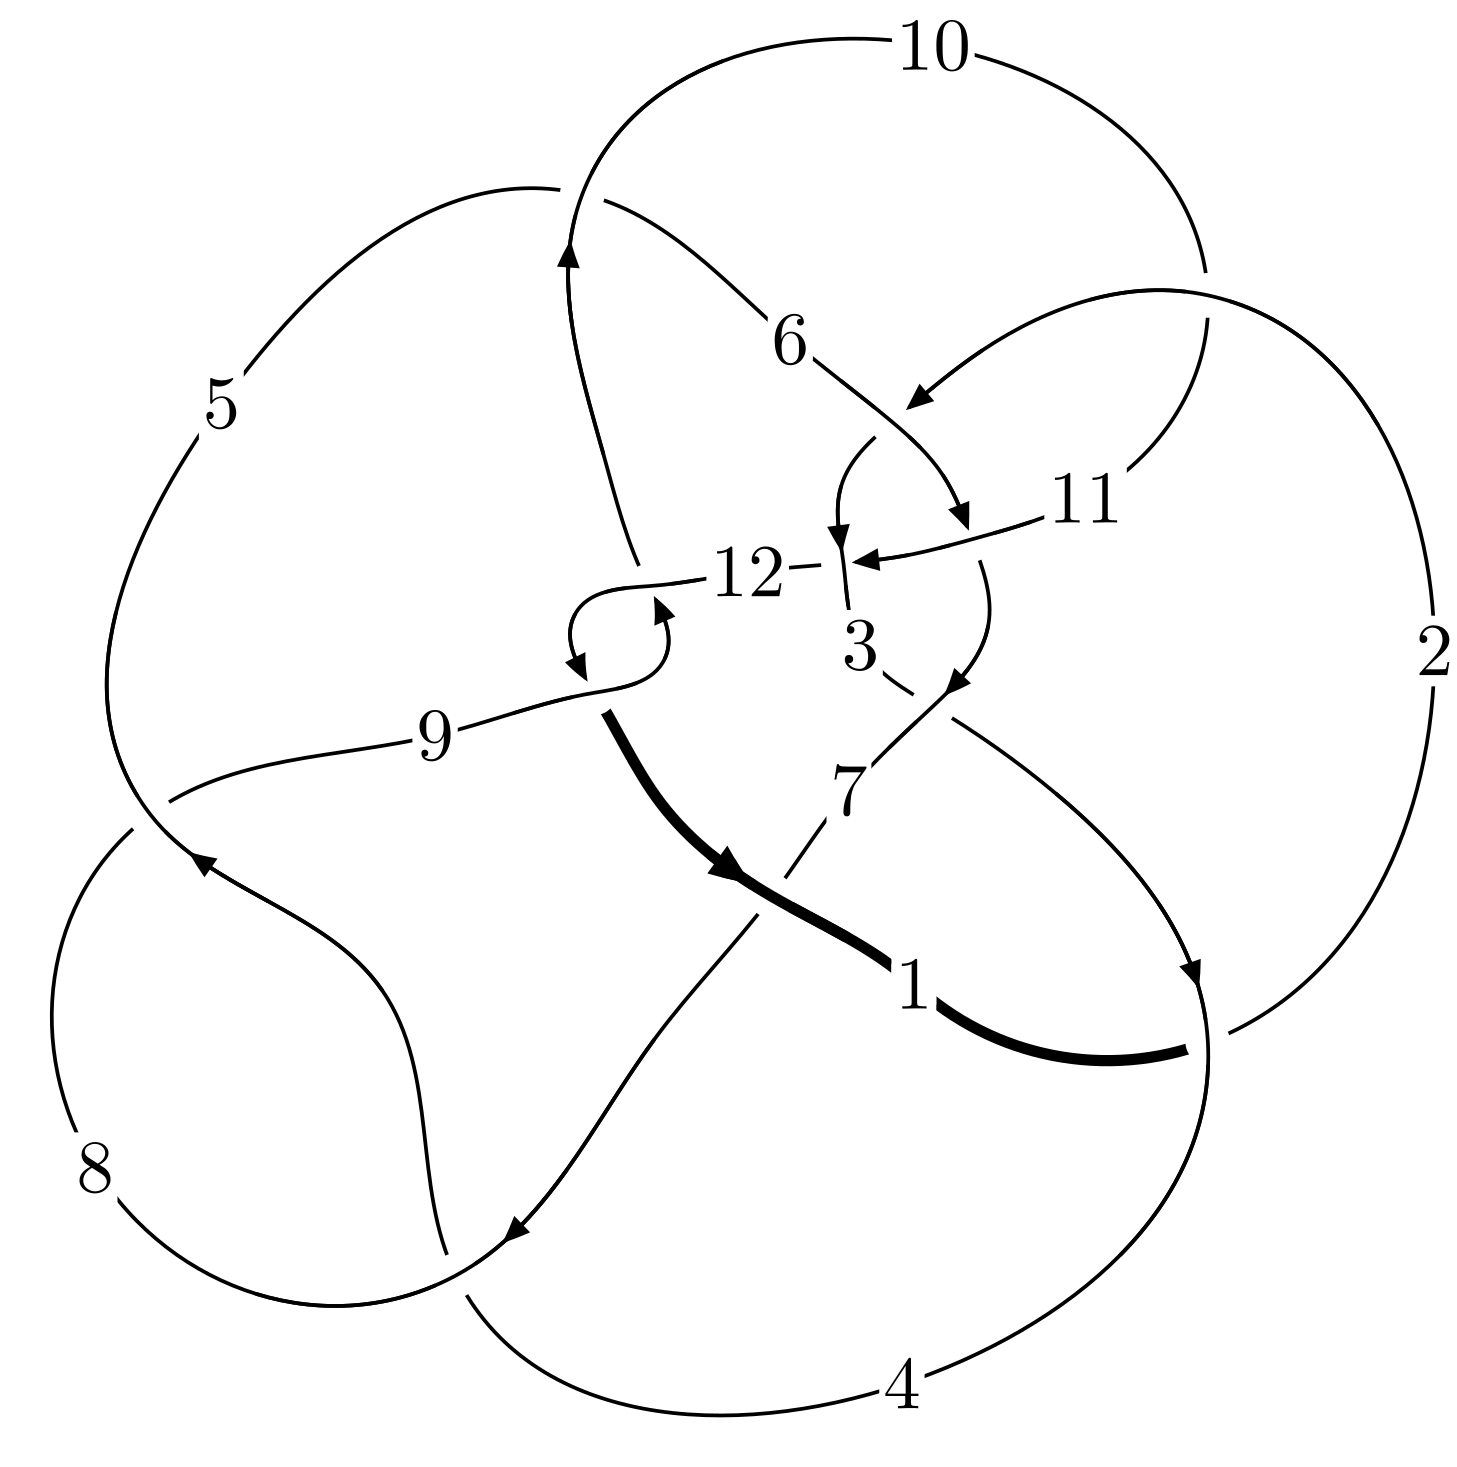
\includegraphics[width=112pt]{../../../GIT/diagram.site/Diagrams/png/1667_12a_0866.png}\\
\ \ \ A knot diagram\footnotemark}&
\allowdisplaybreaks
\textbf{Linearized knot diagam} \\
\cline{2-2}
 &
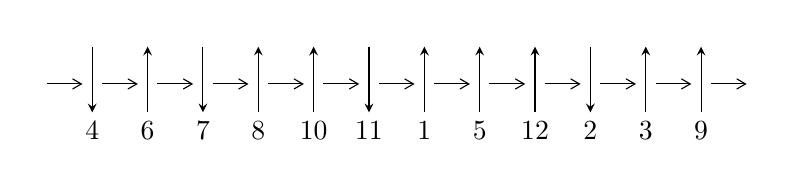
\begin{tikzpicture}[x=20pt, y=17pt]
	% nodes
	\node (C0) at (0, 0) {};
	\node (C1) at (1, 0) {};
	\node (C1U) at (1, +1) {};
	\node (C1D) at (1, -1) {4};

	\node (C2) at (2, 0) {};
	\node (C2U) at (2, +1) {};
	\node (C2D) at (2, -1) {6};

	\node (C3) at (3, 0) {};
	\node (C3U) at (3, +1) {};
	\node (C3D) at (3, -1) {7};

	\node (C4) at (4, 0) {};
	\node (C4U) at (4, +1) {};
	\node (C4D) at (4, -1) {8};

	\node (C5) at (5, 0) {};
	\node (C5U) at (5, +1) {};
	\node (C5D) at (5, -1) {10};

	\node (C6) at (6, 0) {};
	\node (C6U) at (6, +1) {};
	\node (C6D) at (6, -1) {11};

	\node (C7) at (7, 0) {};
	\node (C7U) at (7, +1) {};
	\node (C7D) at (7, -1) {1};

	\node (C8) at (8, 0) {};
	\node (C8U) at (8, +1) {};
	\node (C8D) at (8, -1) {5};

	\node (C9) at (9, 0) {};
	\node (C9U) at (9, +1) {};
	\node (C9D) at (9, -1) {12};

	\node (C10) at (10, 0) {};
	\node (C10U) at (10, +1) {};
	\node (C10D) at (10, -1) {2};

	\node (C11) at (11, 0) {};
	\node (C11U) at (11, +1) {};
	\node (C11D) at (11, -1) {3};

	\node (C12) at (12, 0) {};
	\node (C12U) at (12, +1) {};
	\node (C12D) at (12, -1) {9};
	\node (C13) at (13, 0) {};

	% arrows
	\draw[->,>={angle 60}]
	(C0) edge (C1) (C1) edge (C2) (C2) edge (C3) (C3) edge (C4) (C4) edge (C5) (C5) edge (C6) (C6) edge (C7) (C7) edge (C8) (C8) edge (C9) (C9) edge (C10) (C10) edge (C11) (C11) edge (C12) (C12) edge (C13) ;	\draw[->,>=stealth]
	(C1U) edge (C1D) (C2D) edge (C2U) (C3U) edge (C3D) (C4D) edge (C4U) (C5D) edge (C5U) (C6U) edge (C6D) (C7D) edge (C7U) (C8D) edge (C8U) (C9D) edge (C9U) (C10U) edge (C10D) (C11D) edge (C11U) (C12D) edge (C12U) ;
	\end{tikzpicture} \\
\hhline{~~} \\& 
\textbf{Solving Sequence} \\ \cline{2-2} 
 &
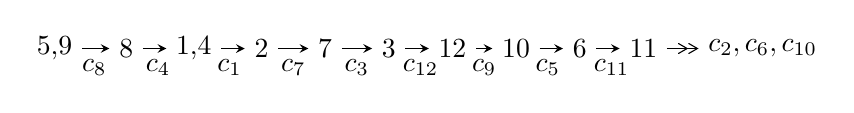
\begin{tikzpicture}[x=23pt, y=7pt]
	% node
	\node (A0) at (-1/8, 0) {5,9};
	\node (A1) at (1, 0) {8};
	\node (A2) at (33/16, 0) {1,4};
	\node (A3) at (25/8, 0) {2};
	\node (A4) at (33/8, 0) {7};
	\node (A5) at (41/8, 0) {3};
	\node (A6) at (49/8, 0) {12};
	\node (A7) at (57/8, 0) {10};
	\node (A8) at (65/8, 0) {6};
	\node (A9) at (73/8, 0) {11};
	\node (C1) at (1/2, -1) {$c_{8}$};
	\node (C2) at (3/2, -1) {$c_{4}$};
	\node (C3) at (21/8, -1) {$c_{1}$};
	\node (C4) at (29/8, -1) {$c_{7}$};
	\node (C5) at (37/8, -1) {$c_{3}$};
	\node (C6) at (45/8, -1) {$c_{12}$};
	\node (C7) at (53/8, -1) {$c_{9}$};
	\node (C8) at (61/8, -1) {$c_{5}$};
	\node (C9) at (69/8, -1) {$c_{11}$};
	\node (A10) at (11, 0) {$c_{2},c_{6},c_{10}$};

	% edge
	\draw[->,>=stealth]	
	(A0) edge (A1) (A1) edge (A2) (A2) edge (A3) (A3) edge (A4) (A4) edge (A5) (A5) edge (A6) (A6) edge (A7) (A7) edge (A8) (A8) edge (A9) ;
	\draw[->>,>={angle 60}]	
	(A9) edge (A10);
\end{tikzpicture} \\ 

\end{tabular} \\

\footnotetext{
The image of knot diagram is generated by the software ``\textbf{Draw programme}" developed by Andrew Bartholomew(\url{http://www.layer8.co.uk/maths/draw/index.htm\#Running-draw}), where we modified some parts for our purpose(\url{https://github.com/CATsTAILs/LinksPainter}).
}\phantom \\ \newline 
\centering \textbf{Ideals for irreducible components\footnotemark of $X_{\text{par}}$} 
 
\begin{align*}
I^u_{1}&=\langle 
1.24767\times10^{1341} u^{187}-6.06121\times10^{1341} u^{186}+\cdots+1.20162\times10^{1340} b-1.42251\times10^{1344},\\
\phantom{I^u_{1}}&\phantom{= \langle  }-1.08645\times10^{1344} u^{187}+5.42636\times10^{1344} u^{186}+\cdots+1.18840\times10^{1343} a+1.08070\times10^{1347},\\
\phantom{I^u_{1}}&\phantom{= \langle  }u^{188}-4 u^{187}+\cdots+7531 u-989\rangle \\
I^u_{2}&=\langle 
5.47253\times10^{48} u^{40}+2.46107\times10^{49} u^{39}+\cdots+2.70094\times10^{48} b-2.27197\times10^{49},\\
\phantom{I^u_{2}}&\phantom{= \langle  }5.87231\times10^{49} u^{40}+3.06842\times10^{50} u^{39}+\cdots+1.35047\times10^{49} a+1.26775\times10^{50},\;u^{41}+5 u^{40}+\cdots+17 u-5\rangle \\
\\
\end{align*}
\raggedright * 2 irreducible components of $\dim_{\mathbb{C}}=0$, with total 229 representations.\\
\footnotetext{All coefficients of polynomials are rational numbers. But the coefficients are sometimes approximated in decimal forms when there is not enough margin.}
\newpage
\renewcommand{\arraystretch}{1}
\centering \section*{I. $I^u_{1}= \langle 1.25\times10^{1341} u^{187}-6.06\times10^{1341} u^{186}+\cdots+1.20\times10^{1340} b-1.42\times10^{1344},\;-1.09\times10^{1344} u^{187}+5.43\times10^{1344} u^{186}+\cdots+1.19\times10^{1343} a+1.08\times10^{1347},\;u^{188}-4 u^{187}+\cdots+7531 u-989 \rangle$}
\flushleft \textbf{(i) Arc colorings}\\
\begin{tabular}{m{7pt} m{180pt} m{7pt} m{180pt} }
\flushright $a_{5}=$&$\begin{pmatrix}0\\u\end{pmatrix}$ \\
\flushright $a_{9}=$&$\begin{pmatrix}1\\0\end{pmatrix}$ \\
\flushright $a_{8}=$&$\begin{pmatrix}1\\u^2\end{pmatrix}$ \\
\flushright $a_{1}=$&$\begin{pmatrix}9.14209 u^{187}-45.6610 u^{186}+\cdots+77974.1 u-9093.73\\-10.3833 u^{187}+50.4421 u^{186}+\cdots-103634. u+11838.3\end{pmatrix}$ \\
\flushright $a_{4}=$&$\begin{pmatrix}- u\\- u^3+u\end{pmatrix}$ \\
\flushright $a_{2}=$&$\begin{pmatrix}16.1336 u^{187}-79.2255 u^{186}+\cdots+152087. u-17506.2\\-13.0510 u^{187}+63.5393 u^{186}+\cdots-128670. u+14714.0\end{pmatrix}$ \\
\flushright $a_{7}=$&$\begin{pmatrix}4.81314 u^{187}-19.8634 u^{186}+\cdots+85954.6 u-9389.88\\-27.3580 u^{187}+135.878 u^{186}+\cdots-241043. u+27898.5\end{pmatrix}$ \\
\flushright $a_{3}=$&$\begin{pmatrix}-91.1154 u^{187}+440.842 u^{186}+\cdots-922623. u+105239.\\-29.3795 u^{187}+141.566 u^{186}+\cdots-304669. u+34670.2\end{pmatrix}$ \\
\flushright $a_{12}=$&$\begin{pmatrix}19.5253 u^{187}-96.1031 u^{186}+\cdots+181608. u-20932.0\\-10.3833 u^{187}+50.4421 u^{186}+\cdots-103634. u+11838.3\end{pmatrix}$ \\
\flushright $a_{10}=$&$\begin{pmatrix}-26.9895 u^{187}+133.796 u^{186}+\cdots-240679. u+27819.1\\32.6104 u^{187}-161.781 u^{186}+\cdots+288032. u-33339.2\end{pmatrix}$ \\
\flushright $a_{6}=$&$\begin{pmatrix}-7.02113 u^{187}+30.1516 u^{186}+\cdots-112632. u+12396.8\\35.4198 u^{187}-173.953 u^{186}+\cdots+332397. u-38206.8\end{pmatrix}$ \\
\flushright $a_{11}=$&$\begin{pmatrix}-28.6648 u^{187}+141.794 u^{186}+\cdots-257959. u+29772.2\\8.27554 u^{187}-41.9809 u^{186}+\cdots+63753.9 u-7503.36\end{pmatrix}$\\&\end{tabular}
\flushleft \textbf{(ii) Obstruction class $= -1$}\\~\\
\flushleft \textbf{(iii) Cusp Shapes $= -481.352 u^{187}+2357.49 u^{186}+\cdots-4.57027\times10^{6} u+524827.$}\\~\\
\newpage\renewcommand{\arraystretch}{1}
\flushleft \textbf{(iv) u-Polynomials at the component}\newline \\
\begin{tabular}{m{50pt}|m{274pt}}
Crossings & \hspace{64pt}u-Polynomials at each crossing \\
\hline $$\begin{aligned}c_{1}\end{aligned}$$&$\begin{aligned}
&u^{188}+6 u^{187}+\cdots-20266 u+1447
\end{aligned}$\\
\hline $$\begin{aligned}c_{2}\end{aligned}$$&$\begin{aligned}
&u^{188}-10 u^{187}+\cdots+235 u+43
\end{aligned}$\\
\hline $$\begin{aligned}c_{3}\end{aligned}$$&$\begin{aligned}
&u^{188}-2 u^{187}+\cdots+2896580 u-507209
\end{aligned}$\\
\hline $$\begin{aligned}c_{4},c_{8}\end{aligned}$$&$\begin{aligned}
&u^{188}+4 u^{187}+\cdots-7531 u-989
\end{aligned}$\\
\hline $$\begin{aligned}c_{5}\end{aligned}$$&$\begin{aligned}
&u^{188}+2 u^{187}+\cdots+11973792223 u+765934129
\end{aligned}$\\
\hline $$\begin{aligned}c_{6}\end{aligned}$$&$\begin{aligned}
&u^{188}+u^{187}+\cdots+7 u+1
\end{aligned}$\\
\hline $$\begin{aligned}c_{7}\end{aligned}$$&$\begin{aligned}
&u^{188}+3 u^{187}+\cdots-30 u+1
\end{aligned}$\\
\hline $$\begin{aligned}c_{9},c_{12}\end{aligned}$$&$\begin{aligned}
&u^{188}-7 u^{187}+\cdots+192850 u+10363
\end{aligned}$\\
\hline $$\begin{aligned}c_{10}\end{aligned}$$&$\begin{aligned}
&u^{188}+6 u^{187}+\cdots+410 u-76
\end{aligned}$\\
\hline $$\begin{aligned}c_{11}\end{aligned}$$&$\begin{aligned}
&u^{188}- u^{187}+\cdots+41 u+1
\end{aligned}$\\
\hline
\end{tabular}\\~\\
\newpage\renewcommand{\arraystretch}{1}
\flushleft \textbf{(v) Riley Polynomials at the component}\newline \\
\begin{tabular}{m{50pt}|m{274pt}}
Crossings & \hspace{64pt}Riley Polynomials at each crossing \\
\hline $$\begin{aligned}c_{1}\end{aligned}$$&$\begin{aligned}
&y^{188}+40 y^{187}+\cdots-47377738 y+2093809
\end{aligned}$\\
\hline $$\begin{aligned}c_{2}\end{aligned}$$&$\begin{aligned}
&y^{188}+8 y^{187}+\cdots-114049 y+1849
\end{aligned}$\\
\hline $$\begin{aligned}c_{3}\end{aligned}$$&$\begin{aligned}
&y^{188}-58 y^{187}+\cdots+8743433592384 y+257260969681
\end{aligned}$\\
\hline $$\begin{aligned}c_{4},c_{8}\end{aligned}$$&$\begin{aligned}
&y^{188}-128 y^{187}+\cdots-18934183 y+978121
\end{aligned}$\\
\hline $$\begin{aligned}c_{5}\end{aligned}$$&$\begin{aligned}
&y^{188}-48 y^{187}+\cdots+2.08\times10^{18} y+5.87\times10^{17}
\end{aligned}$\\
\hline $$\begin{aligned}c_{6}\end{aligned}$$&$\begin{aligned}
&y^{188}-27 y^{187}+\cdots+57 y+1
\end{aligned}$\\
\hline $$\begin{aligned}c_{7}\end{aligned}$$&$\begin{aligned}
&y^{188}+5 y^{187}+\cdots-2302 y+1
\end{aligned}$\\
\hline $$\begin{aligned}c_{9},c_{12}\end{aligned}$$&$\begin{aligned}
&y^{188}+125 y^{187}+\cdots-9867145482 y+107391769
\end{aligned}$\\
\hline $$\begin{aligned}c_{10}\end{aligned}$$&$\begin{aligned}
&y^{188}+22 y^{187}+\cdots-151228 y+5776
\end{aligned}$\\
\hline $$\begin{aligned}c_{11}\end{aligned}$$&$\begin{aligned}
&y^{188}+29 y^{187}+\cdots-229 y+1
\end{aligned}$\\
\hline
\end{tabular}\\~\\
\newpage\flushleft \textbf{(vi) Complex Volumes and Cusp Shapes}
$$\begin{array}{c|c|c}  
\text{Solutions to }I^u_{1}& \I (\text{vol} + \sqrt{-1}CS) & \text{Cusp shape}\\
 \hline 
\begin{aligned}
u &= -0.932910 + 0.374890 I \\
a &= \phantom{-}1.93328 + 0.53959 I \\
b &= \phantom{-}1.123310 - 0.276983 I\end{aligned}
 & \phantom{-}0.26621 + 1.83399 I & \phantom{-0.000000 } 0 \\ \hline\begin{aligned}
u &= -0.932910 - 0.374890 I \\
a &= \phantom{-}1.93328 - 0.53959 I \\
b &= \phantom{-}1.123310 + 0.276983 I\end{aligned}
 & \phantom{-}0.26621 - 1.83399 I & \phantom{-0.000000 } 0 \\ \hline\begin{aligned}
u &= -0.996598 + 0.144886 I \\
a &= -2.37463 - 0.07204 I \\
b &= -0.661471 + 1.177300 I\end{aligned}
 & \phantom{-}1.61320 - 3.13498 I & \phantom{-0.000000 } 0 \\ \hline\begin{aligned}
u &= -0.996598 - 0.144886 I \\
a &= -2.37463 + 0.07204 I \\
b &= -0.661471 - 1.177300 I\end{aligned}
 & \phantom{-}1.61320 + 3.13498 I & \phantom{-0.000000 } 0 \\ \hline\begin{aligned}
u &= \phantom{-}0.800663 + 0.583733 I \\
a &= \phantom{-}1.197290 + 0.283815 I \\
b &= \phantom{-}0.082533 + 0.797857 I\end{aligned}
 & -2.64474 - 0.80224 I & \phantom{-0.000000 } 0 \\ \hline\begin{aligned}
u &= \phantom{-}0.800663 - 0.583733 I \\
a &= \phantom{-}1.197290 - 0.283815 I \\
b &= \phantom{-}0.082533 - 0.797857 I\end{aligned}
 & -2.64474 + 0.80224 I & \phantom{-0.000000 } 0 \\ \hline\begin{aligned}
u &= \phantom{-}0.280613 + 0.974237 I \\
a &= -0.195986 + 0.061527 I \\
b &= -0.297082 - 1.268980 I\end{aligned}
 & -4.21564 + 6.12609 I & \phantom{-0.000000 } 0 \\ \hline\begin{aligned}
u &= \phantom{-}0.280613 - 0.974237 I \\
a &= -0.195986 - 0.061527 I \\
b &= -0.297082 + 1.268980 I\end{aligned}
 & -4.21564 - 6.12609 I & \phantom{-0.000000 } 0 \\ \hline\begin{aligned}
u &= -0.953703 + 0.344085 I \\
a &= -2.58886 - 0.58396 I \\
b &= -0.191327 + 0.971063 I\end{aligned}
 & -0.56636 - 3.02247 I & \phantom{-0.000000 } 0 \\ \hline\begin{aligned}
u &= -0.953703 - 0.344085 I \\
a &= -2.58886 + 0.58396 I \\
b &= -0.191327 - 0.971063 I\end{aligned}
 & -0.56636 + 3.02247 I & \phantom{-0.000000 } 0\\
 \hline 
 \end{array}$$\newpage$$\begin{array}{c|c|c}  
\text{Solutions to }I^u_{1}& \I (\text{vol} + \sqrt{-1}CS) & \text{Cusp shape}\\
 \hline 
\begin{aligned}
u &= \phantom{-}0.172844 + 0.966991 I \\
a &= \phantom{-}0.0155280 - 0.0442956 I \\
b &= -0.626328 + 0.656072 I\end{aligned}
 & -0.12719 - 4.04432 I & \phantom{-0.000000 } 0 \\ \hline\begin{aligned}
u &= \phantom{-}0.172844 - 0.966991 I \\
a &= \phantom{-}0.0155280 + 0.0442956 I \\
b &= -0.626328 - 0.656072 I\end{aligned}
 & -0.12719 + 4.04432 I & \phantom{-0.000000 } 0 \\ \hline\begin{aligned}
u &= \phantom{-}0.736916 + 0.723769 I \\
a &= \phantom{-}0.000229 - 0.277822 I \\
b &= \phantom{-}0.366600 - 1.164660 I\end{aligned}
 & -4.93759 + 1.08711 I & \phantom{-0.000000 } 0 \\ \hline\begin{aligned}
u &= \phantom{-}0.736916 - 0.723769 I \\
a &= \phantom{-}0.000229 + 0.277822 I \\
b &= \phantom{-}0.366600 + 1.164660 I\end{aligned}
 & -4.93759 - 1.08711 I & \phantom{-0.000000 } 0 \\ \hline\begin{aligned}
u &= -0.609610 + 0.748627 I \\
a &= -0.262180 + 0.497281 I \\
b &= \phantom{-}0.497626 + 1.308700 I\end{aligned}
 & -3.68931 + 7.69977 I & \phantom{-0.000000 } 0 \\ \hline\begin{aligned}
u &= -0.609610 - 0.748627 I \\
a &= -0.262180 - 0.497281 I \\
b &= \phantom{-}0.497626 - 1.308700 I\end{aligned}
 & -3.68931 - 7.69977 I & \phantom{-0.000000 } 0 \\ \hline\begin{aligned}
u &= -1.038000 + 0.080493 I \\
a &= \phantom{-}2.46547 + 0.95386 I \\
b &= \phantom{-}0.179638 - 1.089340 I\end{aligned}
 & \phantom{-}0.30068 - 2.24515 I & \phantom{-0.000000 } 0 \\ \hline\begin{aligned}
u &= -1.038000 - 0.080493 I \\
a &= \phantom{-}2.46547 - 0.95386 I \\
b &= \phantom{-}0.179638 + 1.089340 I\end{aligned}
 & \phantom{-}0.30068 + 2.24515 I & \phantom{-0.000000 } 0 \\ \hline\begin{aligned}
u &= -0.953690 + 0.069302 I \\
a &= -2.55229 + 2.99071 I \\
b &= -0.062350 + 0.903689 I\end{aligned}
 & -0.07109 + 1.84615 I & \phantom{-0.000000 } 0 \\ \hline\begin{aligned}
u &= -0.953690 - 0.069302 I \\
a &= -2.55229 - 2.99071 I \\
b &= -0.062350 - 0.903689 I\end{aligned}
 & -0.07109 - 1.84615 I & \phantom{-0.000000 } 0\\
 \hline 
 \end{array}$$\newpage$$\begin{array}{c|c|c}  
\text{Solutions to }I^u_{1}& \I (\text{vol} + \sqrt{-1}CS) & \text{Cusp shape}\\
 \hline 
\begin{aligned}
u &= \phantom{-}0.247844 + 0.918350 I \\
a &= \phantom{-}0.171410 + 0.124767 I \\
b &= \phantom{-}0.380055 - 1.188200 I\end{aligned}
 & -5.72199 - 3.82704 I & \phantom{-0.000000 } 0 \\ \hline\begin{aligned}
u &= \phantom{-}0.247844 - 0.918350 I \\
a &= \phantom{-}0.171410 - 0.124767 I \\
b &= \phantom{-}0.380055 + 1.188200 I\end{aligned}
 & -5.72199 + 3.82704 I & \phantom{-0.000000 } 0 \\ \hline\begin{aligned}
u &= \phantom{-}1.016160 + 0.279333 I \\
a &= -1.32792 - 1.12807 I \\
b &= -0.318385 - 1.351560 I\end{aligned}
 & -4.11608 + 5.09222 I & \phantom{-0.000000 } 0 \\ \hline\begin{aligned}
u &= \phantom{-}1.016160 - 0.279333 I \\
a &= -1.32792 + 1.12807 I \\
b &= -0.318385 + 1.351560 I\end{aligned}
 & -4.11608 - 5.09222 I & \phantom{-0.000000 } 0 \\ \hline\begin{aligned}
u &= -0.942738 + 0.076772 I \\
a &= \phantom{-}0.24442 + 1.97437 I \\
b &= \phantom{-}0.37388 + 2.54242 I\end{aligned}
 & -2.69291 - 5.56907 I & \phantom{-0.000000 } 0 \\ \hline\begin{aligned}
u &= -0.942738 - 0.076772 I \\
a &= \phantom{-}0.24442 - 1.97437 I \\
b &= \phantom{-}0.37388 - 2.54242 I\end{aligned}
 & -2.69291 + 5.56907 I & \phantom{-0.000000 } 0 \\ \hline\begin{aligned}
u &= -0.931386 + 0.164279 I \\
a &= \phantom{-}1.50354 - 1.63984 I \\
b &= \phantom{-}0.84771 - 1.76028 I\end{aligned}
 & -2.47084 + 4.49392 I & \phantom{-0.000000 } 0 \\ \hline\begin{aligned}
u &= -0.931386 - 0.164279 I \\
a &= \phantom{-}1.50354 + 1.63984 I \\
b &= \phantom{-}0.84771 + 1.76028 I\end{aligned}
 & -2.47084 - 4.49392 I & \phantom{-0.000000 } 0 \\ \hline\begin{aligned}
u &= \phantom{-}1.016610 + 0.300180 I \\
a &= -1.60567 - 0.80847 I \\
b &= -0.80045 - 1.66492 I\end{aligned}
 & \phantom{-}0.40390 + 5.46386 I & \phantom{-0.000000 } 0 \\ \hline\begin{aligned}
u &= \phantom{-}1.016610 - 0.300180 I \\
a &= -1.60567 + 0.80847 I \\
b &= -0.80045 + 1.66492 I\end{aligned}
 & \phantom{-}0.40390 - 5.46386 I & \phantom{-0.000000 } 0\\
 \hline 
 \end{array}$$\newpage$$\begin{array}{c|c|c}  
\text{Solutions to }I^u_{1}& \I (\text{vol} + \sqrt{-1}CS) & \text{Cusp shape}\\
 \hline 
\begin{aligned}
u &= -0.931355 + 0.126822 I \\
a &= -1.14362 - 2.09217 I \\
b &= -0.433763 + 0.940358 I\end{aligned}
 & \phantom{-}1.27100 - 2.30835 I & \phantom{-0.000000 } 0 \\ \hline\begin{aligned}
u &= -0.931355 - 0.126822 I \\
a &= -1.14362 + 2.09217 I \\
b &= -0.433763 - 0.940358 I\end{aligned}
 & \phantom{-}1.27100 + 2.30835 I & \phantom{-0.000000 } 0 \\ \hline\begin{aligned}
u &= -0.928997 + 0.042924 I \\
a &= -2.65896 + 0.58032 I \\
b &= -0.235262 - 1.034350 I\end{aligned}
 & -0.32335 - 2.05968 I & \phantom{-0.000000 } 0 \\ \hline\begin{aligned}
u &= -0.928997 - 0.042924 I \\
a &= -2.65896 - 0.58032 I \\
b &= -0.235262 + 1.034350 I\end{aligned}
 & -0.32335 + 2.05968 I & \phantom{-0.000000 } 0 \\ \hline\begin{aligned}
u &= -0.942354 + 0.524880 I \\
a &= \phantom{-}1.80087 - 0.11794 I \\
b &= \phantom{-}0.86557 - 1.30655 I\end{aligned}
 & -2.65383 - 12.54390 I & \phantom{-0.000000 } 0 \\ \hline\begin{aligned}
u &= -0.942354 - 0.524880 I \\
a &= \phantom{-}1.80087 + 0.11794 I \\
b &= \phantom{-}0.86557 + 1.30655 I\end{aligned}
 & -2.65383 + 12.54390 I & \phantom{-0.000000 } 0 \\ \hline\begin{aligned}
u &= -0.417946 + 1.000310 I \\
a &= \phantom{-}0.027120 - 0.411580 I \\
b &= \phantom{-}0.275988 + 0.383954 I\end{aligned}
 & \phantom{-}2.18370 - 2.82632 I & \phantom{-0.000000 } 0 \\ \hline\begin{aligned}
u &= -0.417946 - 1.000310 I \\
a &= \phantom{-}0.027120 + 0.411580 I \\
b &= \phantom{-}0.275988 - 0.383954 I\end{aligned}
 & \phantom{-}2.18370 + 2.82632 I & \phantom{-0.000000 } 0 \\ \hline\begin{aligned}
u &= \phantom{-}1.057050 + 0.242918 I \\
a &= -1.070400 - 0.144920 I \\
b &= -0.39783 - 1.39628 I\end{aligned}
 & \phantom{-}1.05193 + 5.23933 I & \phantom{-0.000000 } 0 \\ \hline\begin{aligned}
u &= \phantom{-}1.057050 - 0.242918 I \\
a &= -1.070400 + 0.144920 I \\
b &= -0.39783 + 1.39628 I\end{aligned}
 & \phantom{-}1.05193 - 5.23933 I & \phantom{-0.000000 } 0\\
 \hline 
 \end{array}$$\newpage$$\begin{array}{c|c|c}  
\text{Solutions to }I^u_{1}& \I (\text{vol} + \sqrt{-1}CS) & \text{Cusp shape}\\
 \hline 
\begin{aligned}
u &= \phantom{-}0.237227 + 0.882104 I \\
a &= -0.354769 - 0.663091 I \\
b &= -0.12411 + 1.42857 I\end{aligned}
 & -6.92090 - 6.38065 I & \phantom{-0.000000 } 0 \\ \hline\begin{aligned}
u &= \phantom{-}0.237227 - 0.882104 I \\
a &= -0.354769 + 0.663091 I \\
b &= -0.12411 - 1.42857 I\end{aligned}
 & -6.92090 + 6.38065 I & \phantom{-0.000000 } 0 \\ \hline\begin{aligned}
u &= \phantom{-}1.090090 + 0.011000 I \\
a &= \phantom{-}1.160750 - 0.408266 I \\
b &= \phantom{-}0.381844 + 0.959733 I\end{aligned}
 & \phantom{-}3.78101 - 4.02611 I & \phantom{-0.000000 } 0 \\ \hline\begin{aligned}
u &= \phantom{-}1.090090 - 0.011000 I \\
a &= \phantom{-}1.160750 + 0.408266 I \\
b &= \phantom{-}0.381844 - 0.959733 I\end{aligned}
 & \phantom{-}3.78101 + 4.02611 I & \phantom{-0.000000 } 0 \\ \hline\begin{aligned}
u &= \phantom{-}0.914975 + 0.597866 I \\
a &= \phantom{-}1.59622 - 0.03954 I \\
b &= \phantom{-}0.599089 + 1.063460 I\end{aligned}
 & -4.34659 + 4.04045 I & \phantom{-0.000000 } 0 \\ \hline\begin{aligned}
u &= \phantom{-}0.914975 - 0.597866 I \\
a &= \phantom{-}1.59622 + 0.03954 I \\
b &= \phantom{-}0.599089 - 1.063460 I\end{aligned}
 & -4.34659 - 4.04045 I & \phantom{-0.000000 } 0 \\ \hline\begin{aligned}
u &= \phantom{-}1.093010 + 0.065407 I \\
a &= -1.71754 - 0.37225 I \\
b &= -0.809823 - 0.988272 I\end{aligned}
 & \phantom{-}4.18823 + 2.92442 I & \phantom{-0.000000 } 0 \\ \hline\begin{aligned}
u &= \phantom{-}1.093010 - 0.065407 I \\
a &= -1.71754 + 0.37225 I \\
b &= -0.809823 + 0.988272 I\end{aligned}
 & \phantom{-}4.18823 - 2.92442 I & \phantom{-0.000000 } 0 \\ \hline\begin{aligned}
u &= \phantom{-}0.066934 + 1.096880 I \\
a &= \phantom{-}0.412070 + 0.213355 I \\
b &= -0.178244 - 1.170140 I\end{aligned}
 & -4.65014 - 0.13962 I & \phantom{-0.000000 } 0 \\ \hline\begin{aligned}
u &= \phantom{-}0.066934 - 1.096880 I \\
a &= \phantom{-}0.412070 - 0.213355 I \\
b &= -0.178244 + 1.170140 I\end{aligned}
 & -4.65014 + 0.13962 I & \phantom{-0.000000 } 0\\
 \hline 
 \end{array}$$\newpage$$\begin{array}{c|c|c}  
\text{Solutions to }I^u_{1}& \I (\text{vol} + \sqrt{-1}CS) & \text{Cusp shape}\\
 \hline 
\begin{aligned}
u &= \phantom{-}1.093090 + 0.173955 I \\
a &= \phantom{-}2.04200 - 0.48788 I \\
b &= \phantom{-}0.482888 + 1.167770 I\end{aligned}
 & \phantom{-}1.18880 + 11.58080 I & \phantom{-0.000000 } 0 \\ \hline\begin{aligned}
u &= \phantom{-}1.093090 - 0.173955 I \\
a &= \phantom{-}2.04200 + 0.48788 I \\
b &= \phantom{-}0.482888 - 1.167770 I\end{aligned}
 & \phantom{-}1.18880 - 11.58080 I & \phantom{-0.000000 } 0 \\ \hline\begin{aligned}
u &= -0.878264 + 0.721877 I \\
a &= -1.126510 - 0.251981 I \\
b &= -0.515284 + 1.152270 I\end{aligned}
 & -2.79956 - 3.72194 I & \phantom{-0.000000 } 0 \\ \hline\begin{aligned}
u &= -0.878264 - 0.721877 I \\
a &= -1.126510 + 0.251981 I \\
b &= -0.515284 - 1.152270 I\end{aligned}
 & -2.79956 + 3.72194 I & \phantom{-0.000000 } 0 \\ \hline\begin{aligned}
u &= -0.143077 + 0.849929 I \\
a &= \phantom{-}0.242181 - 0.368221 I \\
b &= \phantom{-}0.14744 + 1.41971 I\end{aligned}
 & -8.11135 - 2.13818 I & \phantom{-0.000000 } 0 \\ \hline\begin{aligned}
u &= -0.143077 - 0.849929 I \\
a &= \phantom{-}0.242181 + 0.368221 I \\
b &= \phantom{-}0.14744 - 1.41971 I\end{aligned}
 & -8.11135 + 2.13818 I & \phantom{-0.000000 } 0 \\ \hline\begin{aligned}
u &= \phantom{-}0.793452 + 0.299761 I \\
a &= \phantom{-}1.35201 - 0.73462 I \\
b &= \phantom{-}0.418218 - 0.580742 I\end{aligned}
 & -1.41059 + 3.56442 I & \phantom{-0.000000 } 0 \\ \hline\begin{aligned}
u &= \phantom{-}0.793452 - 0.299761 I \\
a &= \phantom{-}1.35201 + 0.73462 I \\
b &= \phantom{-}0.418218 + 0.580742 I\end{aligned}
 & -1.41059 - 3.56442 I & \phantom{-0.000000 } 0 \\ \hline\begin{aligned}
u &= \phantom{-}0.838506 + 0.050942 I \\
a &= \phantom{-}0.246489 + 0.431691 I \\
b &= -0.05190 + 1.74333 I\end{aligned}
 & -5.30636 - 3.63476 I & \phantom{-0.000000 } 0 \\ \hline\begin{aligned}
u &= \phantom{-}0.838506 - 0.050942 I \\
a &= \phantom{-}0.246489 - 0.431691 I \\
b &= -0.05190 - 1.74333 I\end{aligned}
 & -5.30636 + 3.63476 I & \phantom{-0.000000 } 0\\
 \hline 
 \end{array}$$\newpage$$\begin{array}{c|c|c}  
\text{Solutions to }I^u_{1}& \I (\text{vol} + \sqrt{-1}CS) & \text{Cusp shape}\\
 \hline 
\begin{aligned}
u &= \phantom{-}0.797427 + 0.258233 I \\
a &= \phantom{-}0.69037 - 1.29689 I \\
b &= \phantom{-}0.58984 - 1.47107 I\end{aligned}
 & -2.17733 + 3.18711 I & \phantom{-0.000000 } 0 \\ \hline\begin{aligned}
u &= \phantom{-}0.797427 - 0.258233 I \\
a &= \phantom{-}0.69037 + 1.29689 I \\
b &= \phantom{-}0.58984 + 1.47107 I\end{aligned}
 & -2.17733 - 3.18711 I & \phantom{-0.000000 } 0 \\ \hline\begin{aligned}
u &= \phantom{-}0.038241 + 1.174580 I \\
a &= -0.049450 - 0.293969 I \\
b &= -0.449129 + 1.321610 I\end{aligned}
 & -3.24404 - 6.81988 I & \phantom{-0.000000 } 0 \\ \hline\begin{aligned}
u &= \phantom{-}0.038241 - 1.174580 I \\
a &= -0.049450 + 0.293969 I \\
b &= -0.449129 - 1.321610 I\end{aligned}
 & -3.24404 + 6.81988 I & \phantom{-0.000000 } 0 \\ \hline\begin{aligned}
u &= -0.737573 + 0.344825 I \\
a &= -0.401872 + 0.424727 I \\
b &= -0.542224 + 0.055030 I\end{aligned}
 & \phantom{-}0.314526 + 0.273439 I & \phantom{-0.000000 } 0 \\ \hline\begin{aligned}
u &= -0.737573 - 0.344825 I \\
a &= -0.401872 - 0.424727 I \\
b &= -0.542224 - 0.055030 I\end{aligned}
 & \phantom{-}0.314526 - 0.273439 I & \phantom{-0.000000 } 0 \\ \hline\begin{aligned}
u &= -0.760331 + 0.912279 I \\
a &= -0.700304 - 0.833920 I \\
b &= -0.178329 + 0.739824 I\end{aligned}
 & -1.59398 - 4.71317 I & \phantom{-0.000000 } 0 \\ \hline\begin{aligned}
u &= -0.760331 - 0.912279 I \\
a &= -0.700304 + 0.833920 I \\
b &= -0.178329 - 0.739824 I\end{aligned}
 & -1.59398 + 4.71317 I & \phantom{-0.000000 } 0 \\ \hline\begin{aligned}
u &= -0.792395 + 0.075302 I \\
a &= \phantom{-}1.91632 + 0.06197 I \\
b &= -0.303307 - 0.856990 I\end{aligned}
 & \phantom{-}0.88217 + 1.81809 I & \phantom{-0.000000 } 0 \\ \hline\begin{aligned}
u &= -0.792395 - 0.075302 I \\
a &= \phantom{-}1.91632 - 0.06197 I \\
b &= -0.303307 + 0.856990 I\end{aligned}
 & \phantom{-}0.88217 - 1.81809 I & \phantom{-0.000000 } 0\\
 \hline 
 \end{array}$$\newpage$$\begin{array}{c|c|c}  
\text{Solutions to }I^u_{1}& \I (\text{vol} + \sqrt{-1}CS) & \text{Cusp shape}\\
 \hline 
\begin{aligned}
u &= -0.689860 + 0.992521 I \\
a &= \phantom{-}0.246278 - 0.263116 I \\
b &= -0.267383 - 1.139260 I\end{aligned}
 & -3.48813 - 2.56118 I & \phantom{-0.000000 } 0 \\ \hline\begin{aligned}
u &= -0.689860 - 0.992521 I \\
a &= \phantom{-}0.246278 + 0.263116 I \\
b &= -0.267383 + 1.139260 I\end{aligned}
 & -3.48813 + 2.56118 I & \phantom{-0.000000 } 0 \\ \hline\begin{aligned}
u &= \phantom{-}1.172210 + 0.333764 I \\
a &= -1.166690 + 0.620790 I \\
b &= -1.34470 + 0.69553 I\end{aligned}
 & \phantom{-}4.39351 + 2.17711 I & \phantom{-0.000000 } 0 \\ \hline\begin{aligned}
u &= \phantom{-}1.172210 - 0.333764 I \\
a &= -1.166690 - 0.620790 I \\
b &= -1.34470 - 0.69553 I\end{aligned}
 & \phantom{-}4.39351 - 2.17711 I & \phantom{-0.000000 } 0 \\ \hline\begin{aligned}
u &= -1.055890 + 0.666769 I \\
a &= \phantom{-}0.950237 + 0.098821 I \\
b &= -0.101000 - 0.882782 I\end{aligned}
 & \phantom{-}0.490665 - 0.628637 I & \phantom{-0.000000 } 0 \\ \hline\begin{aligned}
u &= -1.055890 - 0.666769 I \\
a &= \phantom{-}0.950237 - 0.098821 I \\
b &= -0.101000 + 0.882782 I\end{aligned}
 & \phantom{-}0.490665 + 0.628637 I & \phantom{-0.000000 } 0 \\ \hline\begin{aligned}
u &= -1.233300 + 0.221792 I \\
a &= -1.69296 + 0.01656 I \\
b &= -1.376200 - 0.084632 I\end{aligned}
 & \phantom{-}4.86637 - 4.55618 I & \phantom{-0.000000 } 0 \\ \hline\begin{aligned}
u &= -1.233300 - 0.221792 I \\
a &= -1.69296 - 0.01656 I \\
b &= -1.376200 + 0.084632 I\end{aligned}
 & \phantom{-}4.86637 + 4.55618 I & \phantom{-0.000000 } 0 \\ \hline\begin{aligned}
u &= -1.210390 + 0.340081 I \\
a &= -1.011680 + 0.639835 I \\
b &= -0.68903 + 1.48663 I\end{aligned}
 & -0.32590 - 4.89336 I & \phantom{-0.000000 } 0 \\ \hline\begin{aligned}
u &= -1.210390 - 0.340081 I \\
a &= -1.011680 - 0.639835 I \\
b &= -0.68903 - 1.48663 I\end{aligned}
 & -0.32590 + 4.89336 I & \phantom{-0.000000 } 0\\
 \hline 
 \end{array}$$\newpage$$\begin{array}{c|c|c}  
\text{Solutions to }I^u_{1}& \I (\text{vol} + \sqrt{-1}CS) & \text{Cusp shape}\\
 \hline 
\begin{aligned}
u &= -0.042559 + 1.272700 I \\
a &= \phantom{-}0.106273 - 0.199339 I \\
b &= \phantom{-}0.446988 + 1.265610 I\end{aligned}
 & -4.3002 + 15.1636 I & \phantom{-0.000000 } 0 \\ \hline\begin{aligned}
u &= -0.042559 - 1.272700 I \\
a &= \phantom{-}0.106273 + 0.199339 I \\
b &= \phantom{-}0.446988 - 1.265610 I\end{aligned}
 & -4.3002 - 15.1636 I & \phantom{-0.000000 } 0 \\ \hline\begin{aligned}
u &= \phantom{-}1.237330 + 0.318025 I \\
a &= -1.63120 + 0.25335 I \\
b &= -1.51362 - 0.10706 I\end{aligned}
 & \phantom{-}5.69770 + 5.54914 I & \phantom{-0.000000 } 0 \\ \hline\begin{aligned}
u &= \phantom{-}1.237330 - 0.318025 I \\
a &= -1.63120 - 0.25335 I \\
b &= -1.51362 + 0.10706 I\end{aligned}
 & \phantom{-}5.69770 - 5.54914 I & \phantom{-0.000000 } 0 \\ \hline\begin{aligned}
u &= \phantom{-}1.274920 + 0.121531 I \\
a &= -1.328670 + 0.056009 I \\
b &= -1.160930 + 0.104440 I\end{aligned}
 & \phantom{-}6.07502 + 0.48235 I & \phantom{-0.000000 } 0 \\ \hline\begin{aligned}
u &= \phantom{-}1.274920 - 0.121531 I \\
a &= -1.328670 - 0.056009 I \\
b &= -1.160930 - 0.104440 I\end{aligned}
 & \phantom{-}6.07502 - 0.48235 I & \phantom{-0.000000 } 0 \\ \hline\begin{aligned}
u &= \phantom{-}1.225570 + 0.390920 I \\
a &= \phantom{-}1.242890 - 0.270708 I \\
b &= \phantom{-}0.992814 - 0.260230 I\end{aligned}
 & \phantom{-}2.24094 + 7.27695 I & \phantom{-0.000000 } 0 \\ \hline\begin{aligned}
u &= \phantom{-}1.225570 - 0.390920 I \\
a &= \phantom{-}1.242890 + 0.270708 I \\
b &= \phantom{-}0.992814 + 0.260230 I\end{aligned}
 & \phantom{-}2.24094 - 7.27695 I & \phantom{-0.000000 } 0 \\ \hline\begin{aligned}
u &= -1.286800 + 0.063950 I \\
a &= \phantom{-}0.33795 - 1.66749 I \\
b &= -0.144268 - 0.703422 I\end{aligned}
 & \phantom{-}2.39969 + 0.70690 I & \phantom{-0.000000 } 0 \\ \hline\begin{aligned}
u &= -1.286800 - 0.063950 I \\
a &= \phantom{-}0.33795 + 1.66749 I \\
b &= -0.144268 + 0.703422 I\end{aligned}
 & \phantom{-}2.39969 - 0.70690 I & \phantom{-0.000000 } 0\\
 \hline 
 \end{array}$$\newpage$$\begin{array}{c|c|c}  
\text{Solutions to }I^u_{1}& \I (\text{vol} + \sqrt{-1}CS) & \text{Cusp shape}\\
 \hline 
\begin{aligned}
u &= \phantom{-}0.136227 + 1.285270 I \\
a &= \phantom{-}0.173581 + 0.197725 I \\
b &= \phantom{-}0.327236 - 1.141150 I\end{aligned}
 & -4.80765 - 6.38541 I & \phantom{-0.000000 } 0 \\ \hline\begin{aligned}
u &= \phantom{-}0.136227 - 1.285270 I \\
a &= \phantom{-}0.173581 - 0.197725 I \\
b &= \phantom{-}0.327236 + 1.141150 I\end{aligned}
 & -4.80765 + 6.38541 I & \phantom{-0.000000 } 0 \\ \hline\begin{aligned}
u &= \phantom{-}0.702869 + 0.057996 I \\
a &= -2.72893 + 0.77261 I \\
b &= \phantom{-}0.201167 + 0.662724 I\end{aligned}
 & -0.52183 + 10.48050 I & \phantom{-0.000000 } 0 \\ \hline\begin{aligned}
u &= \phantom{-}0.702869 - 0.057996 I \\
a &= -2.72893 - 0.77261 I \\
b &= \phantom{-}0.201167 - 0.662724 I\end{aligned}
 & -0.52183 - 10.48050 I & \phantom{-0.000000 } 0 \\ \hline\begin{aligned}
u &= \phantom{-}1.288290 + 0.163301 I \\
a &= -1.52727 - 0.61324 I \\
b &= -0.964652 - 0.702479 I\end{aligned}
 & \phantom{-}5.08321 + 3.68372 I & \phantom{-0.000000 } 0 \\ \hline\begin{aligned}
u &= \phantom{-}1.288290 - 0.163301 I \\
a &= -1.52727 + 0.61324 I \\
b &= -0.964652 + 0.702479 I\end{aligned}
 & \phantom{-}5.08321 - 3.68372 I & \phantom{-0.000000 } 0 \\ \hline\begin{aligned}
u &= \phantom{-}0.625160 + 0.313756 I \\
a &= \phantom{-}1.92785 + 0.16397 I \\
b &= \phantom{-}0.781365 + 0.542075 I\end{aligned}
 & -2.52291 - 0.24082 I & \phantom{-0.000000 } 0 \\ \hline\begin{aligned}
u &= \phantom{-}0.625160 - 0.313756 I \\
a &= \phantom{-}1.92785 - 0.16397 I \\
b &= \phantom{-}0.781365 - 0.542075 I\end{aligned}
 & -2.52291 + 0.24082 I & \phantom{-0.000000 } 0 \\ \hline\begin{aligned}
u &= -1.275200 + 0.279077 I \\
a &= \phantom{-}1.016160 - 0.230755 I \\
b &= \phantom{-}0.216454 - 0.841733 I\end{aligned}
 & \phantom{-}0.97220 - 1.12401 I & \phantom{-0.000000 } 0 \\ \hline\begin{aligned}
u &= -1.275200 - 0.279077 I \\
a &= \phantom{-}1.016160 + 0.230755 I \\
b &= \phantom{-}0.216454 + 0.841733 I\end{aligned}
 & \phantom{-}0.97220 + 1.12401 I & \phantom{-0.000000 } 0\\
 \hline 
 \end{array}$$\newpage$$\begin{array}{c|c|c}  
\text{Solutions to }I^u_{1}& \I (\text{vol} + \sqrt{-1}CS) & \text{Cusp shape}\\
 \hline 
\begin{aligned}
u &= \phantom{-}1.203870 + 0.514891 I \\
a &= \phantom{-}1.66892 + 0.24257 I \\
b &= \phantom{-}0.669345 + 1.161300 I\end{aligned}
 & -2.72364 + 8.99909 I & \phantom{-0.000000 } 0 \\ \hline\begin{aligned}
u &= \phantom{-}1.203870 - 0.514891 I \\
a &= \phantom{-}1.66892 - 0.24257 I \\
b &= \phantom{-}0.669345 - 1.161300 I\end{aligned}
 & -2.72364 - 8.99909 I & \phantom{-0.000000 } 0 \\ \hline\begin{aligned}
u &= \phantom{-}0.280944 + 0.624914 I \\
a &= -0.397842 + 1.214640 I \\
b &= \phantom{-}0.677791 + 0.115239 I\end{aligned}
 & -0.33402 + 10.82870 I & \phantom{-0.000000 } 0 \\ \hline\begin{aligned}
u &= \phantom{-}0.280944 - 0.624914 I \\
a &= -0.397842 - 1.214640 I \\
b &= \phantom{-}0.677791 - 0.115239 I\end{aligned}
 & -0.33402 - 10.82870 I & \phantom{-0.000000 } 0 \\ \hline\begin{aligned}
u &= -1.313350 + 0.066298 I \\
a &= \phantom{-}0.503375 - 0.445082 I \\
b &= \phantom{-}0.141304 + 0.011398 I\end{aligned}
 & \phantom{-}2.60885 + 0.38010 I & \phantom{-0.000000 } 0 \\ \hline\begin{aligned}
u &= -1.313350 - 0.066298 I \\
a &= \phantom{-}0.503375 + 0.445082 I \\
b &= \phantom{-}0.141304 - 0.011398 I\end{aligned}
 & \phantom{-}2.60885 - 0.38010 I & \phantom{-0.000000 } 0 \\ \hline\begin{aligned}
u &= \phantom{-}1.225930 + 0.487300 I \\
a &= -1.73908 - 0.41691 I \\
b &= -0.255367 - 1.261240 I\end{aligned}
 & -3.78838 + 11.37000 I & \phantom{-0.000000 } 0 \\ \hline\begin{aligned}
u &= \phantom{-}1.225930 - 0.487300 I \\
a &= -1.73908 + 0.41691 I \\
b &= -0.255367 + 1.261240 I\end{aligned}
 & -3.78838 - 11.37000 I & \phantom{-0.000000 } 0 \\ \hline\begin{aligned}
u &= -1.267900 + 0.369952 I \\
a &= \phantom{-}1.45749 + 0.29255 I \\
b &= \phantom{-}1.43189 + 0.09759 I\end{aligned}
 & \phantom{-}4.0219 - 14.5167 I & \phantom{-0.000000 } 0 \\ \hline\begin{aligned}
u &= -1.267900 - 0.369952 I \\
a &= \phantom{-}1.45749 - 0.29255 I \\
b &= \phantom{-}1.43189 - 0.09759 I\end{aligned}
 & \phantom{-}4.0219 + 14.5167 I & \phantom{-0.000000 } 0\\
 \hline 
 \end{array}$$\newpage$$\begin{array}{c|c|c}  
\text{Solutions to }I^u_{1}& \I (\text{vol} + \sqrt{-1}CS) & \text{Cusp shape}\\
 \hline 
\begin{aligned}
u &= -1.243650 + 0.457547 I \\
a &= \phantom{-}1.61596 - 0.57051 I \\
b &= \phantom{-}0.386573 - 1.282890 I\end{aligned}
 & -4.67811 - 2.62718 I & \phantom{-0.000000 } 0 \\ \hline\begin{aligned}
u &= -1.243650 - 0.457547 I \\
a &= \phantom{-}1.61596 + 0.57051 I \\
b &= \phantom{-}0.386573 + 1.282890 I\end{aligned}
 & -4.67811 + 2.62718 I & \phantom{-0.000000 } 0 \\ \hline\begin{aligned}
u &= \phantom{-}1.344450 + 0.052059 I \\
a &= \phantom{-}0.846673 - 0.926095 I \\
b &= \phantom{-}0.685074 - 0.303345 I\end{aligned}
 & \phantom{-}3.82994 + 7.06531 I & \phantom{-0.000000 } 0 \\ \hline\begin{aligned}
u &= \phantom{-}1.344450 - 0.052059 I \\
a &= \phantom{-}0.846673 + 0.926095 I \\
b &= \phantom{-}0.685074 + 0.303345 I\end{aligned}
 & \phantom{-}3.82994 - 7.06531 I & \phantom{-0.000000 } 0 \\ \hline\begin{aligned}
u &= -0.298814 + 0.582284 I \\
a &= \phantom{-}0.501492 + 0.589634 I \\
b &= -0.734903 + 0.253216 I\end{aligned}
 & \phantom{-}1.37252 - 2.34420 I & \phantom{-0.000000 } 0 \\ \hline\begin{aligned}
u &= -0.298814 - 0.582284 I \\
a &= \phantom{-}0.501492 - 0.589634 I \\
b &= -0.734903 - 0.253216 I\end{aligned}
 & \phantom{-}1.37252 + 2.34420 I & \phantom{-0.000000 } 0 \\ \hline\begin{aligned}
u &= \phantom{-}0.524688 + 1.240660 I \\
a &= -0.184972 + 0.491833 I \\
b &= \phantom{-}0.286579 - 0.954381 I\end{aligned}
 & \phantom{-}0.82739 - 5.64505 I & \phantom{-0.000000 } 0 \\ \hline\begin{aligned}
u &= \phantom{-}0.524688 - 1.240660 I \\
a &= -0.184972 - 0.491833 I \\
b &= \phantom{-}0.286579 + 0.954381 I\end{aligned}
 & \phantom{-}0.82739 + 5.64505 I & \phantom{-0.000000 } 0 \\ \hline\begin{aligned}
u &= -1.316870 + 0.332700 I \\
a &= -1.119410 + 0.109239 I \\
b &= -0.970468 - 0.052702 I\end{aligned}
 & \phantom{-}3.41416 - 5.99433 I & \phantom{-0.000000 } 0 \\ \hline\begin{aligned}
u &= -1.316870 - 0.332700 I \\
a &= -1.119410 - 0.109239 I \\
b &= -0.970468 + 0.052702 I\end{aligned}
 & \phantom{-}3.41416 + 5.99433 I & \phantom{-0.000000 } 0\\
 \hline 
 \end{array}$$\newpage$$\begin{array}{c|c|c}  
\text{Solutions to }I^u_{1}& \I (\text{vol} + \sqrt{-1}CS) & \text{Cusp shape}\\
 \hline 
\begin{aligned}
u &= -1.169870 + 0.702461 I \\
a &= \phantom{-}0.872281 + 0.345641 I \\
b &= \phantom{-}0.173247 - 1.099880 I\end{aligned}
 & \phantom{-}0.279407 - 1.380150 I & \phantom{-0.000000 } 0 \\ \hline\begin{aligned}
u &= -1.169870 - 0.702461 I \\
a &= \phantom{-}0.872281 - 0.345641 I \\
b &= \phantom{-}0.173247 + 1.099880 I\end{aligned}
 & \phantom{-}0.279407 + 1.380150 I & \phantom{-0.000000 } 0 \\ \hline\begin{aligned}
u &= -1.335590 + 0.297697 I \\
a &= \phantom{-}0.895012 + 0.271081 I \\
b &= \phantom{-}0.864981 + 0.579635 I\end{aligned}
 & \phantom{-}6.92609 + 1.69202 I & \phantom{-0.000000 } 0 \\ \hline\begin{aligned}
u &= -1.335590 - 0.297697 I \\
a &= \phantom{-}0.895012 - 0.271081 I \\
b &= \phantom{-}0.864981 - 0.579635 I\end{aligned}
 & \phantom{-}6.92609 - 1.69202 I & \phantom{-0.000000 } 0 \\ \hline\begin{aligned}
u &= \phantom{-}0.464000 + 0.412112 I \\
a &= \phantom{-}1.170960 - 0.452696 I \\
b &= \phantom{-}0.555009 - 0.071113 I\end{aligned}
 & -2.20672 - 0.16388 I & \phantom{-0.000000 } 0 \\ \hline\begin{aligned}
u &= \phantom{-}0.464000 - 0.412112 I \\
a &= \phantom{-}1.170960 + 0.452696 I \\
b &= \phantom{-}0.555009 + 0.071113 I\end{aligned}
 & -2.20672 + 0.16388 I & \phantom{-0.000000 } 0 \\ \hline\begin{aligned}
u &= \phantom{-}0.054521 + 0.612898 I \\
a &= \phantom{-}0.801353 - 0.681042 I \\
b &= -0.276445 + 1.160900 I\end{aligned}
 & -1.92177 - 2.72881 I & \phantom{-0.000000 } 0 \\ \hline\begin{aligned}
u &= \phantom{-}0.054521 - 0.612898 I \\
a &= \phantom{-}0.801353 + 0.681042 I \\
b &= -0.276445 - 1.160900 I\end{aligned}
 & -1.92177 + 2.72881 I & \phantom{-0.000000 } 0 \\ \hline\begin{aligned}
u &= \phantom{-}1.262480 + 0.593621 I \\
a &= -1.379590 + 0.129524 I \\
b &= -0.874746 - 1.004710 I\end{aligned}
 & \phantom{-}3.13171 + 9.71662 I & \phantom{-0.000000 } 0 \\ \hline\begin{aligned}
u &= \phantom{-}1.262480 - 0.593621 I \\
a &= -1.379590 - 0.129524 I \\
b &= -0.874746 + 1.004710 I\end{aligned}
 & \phantom{-}3.13171 - 9.71662 I & \phantom{-0.000000 } 0\\
 \hline 
 \end{array}$$\newpage$$\begin{array}{c|c|c}  
\text{Solutions to }I^u_{1}& \I (\text{vol} + \sqrt{-1}CS) & \text{Cusp shape}\\
 \hline 
\begin{aligned}
u &= -0.039229 + 0.602811 I \\
a &= \phantom{-}0.724272 - 1.129440 I \\
b &= \phantom{-}0.455629 - 0.132455 I\end{aligned}
 & -1.45671 - 3.45841 I & \phantom{-0.000000 } 0 \\ \hline\begin{aligned}
u &= -0.039229 - 0.602811 I \\
a &= \phantom{-}0.724272 + 1.129440 I \\
b &= \phantom{-}0.455629 + 0.132455 I\end{aligned}
 & -1.45671 + 3.45841 I & \phantom{-0.000000 } 0 \\ \hline\begin{aligned}
u &= \phantom{-}0.601553\phantom{ +0.000000I} \\
a &= -3.51220\phantom{ +0.000000I} \\
b &= -1.29166\phantom{ +0.000000I}\end{aligned}
 & \phantom{-}1.59492\phantom{ +0.000000I} & \phantom{-0.000000 } 0 \\ \hline\begin{aligned}
u &= -0.322276 + 0.501776 I \\
a &= \phantom{-}0.114286 + 0.849844 I \\
b &= \phantom{-}0.875562 + 0.623564 I\end{aligned}
 & -1.29729 - 5.33922 I & \phantom{-0.000000 } 0 \\ \hline\begin{aligned}
u &= -0.322276 - 0.501776 I \\
a &= \phantom{-}0.114286 - 0.849844 I \\
b &= \phantom{-}0.875562 - 0.623564 I\end{aligned}
 & -1.29729 + 5.33922 I & \phantom{-0.000000 } 0 \\ \hline\begin{aligned}
u &= \phantom{-}1.337300 + 0.426723 I \\
a &= -1.312820 - 0.281781 I \\
b &= -0.62436 - 1.32387 I\end{aligned}
 & \phantom{-}2.29872 + 6.76585 I & \phantom{-0.000000 } 0 \\ \hline\begin{aligned}
u &= \phantom{-}1.337300 - 0.426723 I \\
a &= -1.312820 + 0.281781 I \\
b &= -0.62436 + 1.32387 I\end{aligned}
 & \phantom{-}2.29872 - 6.76585 I & \phantom{-0.000000 } 0 \\ \hline\begin{aligned}
u &= \phantom{-}1.358890 + 0.366542 I \\
a &= \phantom{-}0.942302 - 0.258572 I \\
b &= \phantom{-}0.910493 - 0.158063 I\end{aligned}
 & \phantom{-}7.53133 + 7.30721 I & \phantom{-0.000000 } 0 \\ \hline\begin{aligned}
u &= \phantom{-}1.358890 - 0.366542 I \\
a &= \phantom{-}0.942302 + 0.258572 I \\
b &= \phantom{-}0.910493 + 0.158063 I\end{aligned}
 & \phantom{-}7.53133 - 7.30721 I & \phantom{-0.000000 } 0 \\ \hline\begin{aligned}
u &= \phantom{-}1.054390 + 0.938320 I \\
a &= \phantom{-}0.789677 - 0.214326 I \\
b &= \phantom{-}0.119978 + 0.787453 I\end{aligned}
 & -2.91575 + 3.65835 I & \phantom{-0.000000 } 0\\
 \hline 
 \end{array}$$\newpage$$\begin{array}{c|c|c}  
\text{Solutions to }I^u_{1}& \I (\text{vol} + \sqrt{-1}CS) & \text{Cusp shape}\\
 \hline 
\begin{aligned}
u &= \phantom{-}1.054390 - 0.938320 I \\
a &= \phantom{-}0.789677 + 0.214326 I \\
b &= \phantom{-}0.119978 - 0.787453 I\end{aligned}
 & -2.91575 - 3.65835 I & \phantom{-0.000000 } 0 \\ \hline\begin{aligned}
u &= -0.540970 + 0.215038 I \\
a &= \phantom{-}2.19712 + 0.25264 I \\
b &= -0.340833 - 0.221987 I\end{aligned}
 & \phantom{-}0.803133 + 0.043679 I & \phantom{-0.000000 } 0 \\ \hline\begin{aligned}
u &= -0.540970 - 0.215038 I \\
a &= \phantom{-}2.19712 - 0.25264 I \\
b &= -0.340833 + 0.221987 I\end{aligned}
 & \phantom{-}0.803133 - 0.043679 I & \phantom{-0.000000 } 0 \\ \hline\begin{aligned}
u &= \phantom{-}1.28045 + 0.60963 I \\
a &= \phantom{-}1.158220 + 0.241375 I \\
b &= \phantom{-}0.138029 + 0.859303 I\end{aligned}
 & -0.94409 + 6.18960 I & \phantom{-0.000000 } 0 \\ \hline\begin{aligned}
u &= \phantom{-}1.28045 - 0.60963 I \\
a &= \phantom{-}1.158220 - 0.241375 I \\
b &= \phantom{-}0.138029 - 0.859303 I\end{aligned}
 & -0.94409 - 6.18960 I & \phantom{-0.000000 } 0 \\ \hline\begin{aligned}
u &= -1.39339 + 0.30307 I \\
a &= -0.742021 - 0.265368 I \\
b &= -0.995971 - 0.080948 I\end{aligned}
 & \phantom{-}5.02981 - 0.81679 I & \phantom{-0.000000 } 0 \\ \hline\begin{aligned}
u &= -1.39339 - 0.30307 I \\
a &= -0.742021 + 0.265368 I \\
b &= -0.995971 + 0.080948 I\end{aligned}
 & \phantom{-}5.02981 + 0.81679 I & \phantom{-0.000000 } 0 \\ \hline\begin{aligned}
u &= \phantom{-}0.15925 + 1.41721 I \\
a &= -0.0599314 + 0.1206730 I \\
b &= -0.238860 - 1.170030 I\end{aligned}
 & -5.41255 + 4.51169 I & \phantom{-0.000000 } 0 \\ \hline\begin{aligned}
u &= \phantom{-}0.15925 - 1.41721 I \\
a &= -0.0599314 - 0.1206730 I \\
b &= -0.238860 + 1.170030 I\end{aligned}
 & -5.41255 - 4.51169 I & \phantom{-0.000000 } 0 \\ \hline\begin{aligned}
u &= -1.08163 + 0.97988 I \\
a &= -0.360481 - 0.385020 I \\
b &= -0.289498 + 0.674799 I\end{aligned}
 & \phantom{-}2.46803 - 2.74768 I & \phantom{-0.000000 } 0\\
 \hline 
 \end{array}$$\newpage$$\begin{array}{c|c|c}  
\text{Solutions to }I^u_{1}& \I (\text{vol} + \sqrt{-1}CS) & \text{Cusp shape}\\
 \hline 
\begin{aligned}
u &= -1.08163 - 0.97988 I \\
a &= -0.360481 + 0.385020 I \\
b &= -0.289498 - 0.674799 I\end{aligned}
 & \phantom{-}2.46803 + 2.74768 I & \phantom{-0.000000 } 0 \\ \hline\begin{aligned}
u &= \phantom{-}1.35294 + 0.57563 I \\
a &= -1.46670 - 0.22727 I \\
b &= -0.67192 - 1.47492 I\end{aligned}
 & \phantom{-}0.85959 + 12.91490 I & \phantom{-0.000000 } 0 \\ \hline\begin{aligned}
u &= \phantom{-}1.35294 - 0.57563 I \\
a &= -1.46670 + 0.22727 I \\
b &= -0.67192 + 1.47492 I\end{aligned}
 & \phantom{-}0.85959 - 12.91490 I & \phantom{-0.000000 } 0 \\ \hline\begin{aligned}
u &= -1.35338 + 0.61297 I \\
a &= \phantom{-}1.139680 + 0.050554 I \\
b &= \phantom{-}0.607537 - 1.012880 I\end{aligned}
 & \phantom{-}5.51021 - 3.73980 I & \phantom{-0.000000 } 0 \\ \hline\begin{aligned}
u &= -1.35338 - 0.61297 I \\
a &= \phantom{-}1.139680 - 0.050554 I \\
b &= \phantom{-}0.607537 + 1.012880 I\end{aligned}
 & \phantom{-}5.51021 + 3.73980 I & \phantom{-0.000000 } 0 \\ \hline\begin{aligned}
u &= \phantom{-}1.33863 + 0.65073 I \\
a &= \phantom{-}1.208010 - 0.111880 I \\
b &= \phantom{-}0.516267 + 1.272760 I\end{aligned}
 & \phantom{-}4.03794 + 12.50820 I & \phantom{-0.000000 } 0 \\ \hline\begin{aligned}
u &= \phantom{-}1.33863 - 0.65073 I \\
a &= \phantom{-}1.208010 + 0.111880 I \\
b &= \phantom{-}0.516267 - 1.272760 I\end{aligned}
 & \phantom{-}4.03794 - 12.50820 I & \phantom{-0.000000 } 0 \\ \hline\begin{aligned}
u &= \phantom{-}1.36098 + 0.62304 I \\
a &= \phantom{-}1.370230 + 0.144426 I \\
b &= \phantom{-}0.580599 + 1.251450 I\end{aligned}
 & -0.89606 + 12.95830 I & \phantom{-0.000000 } 0 \\ \hline\begin{aligned}
u &= \phantom{-}1.36098 - 0.62304 I \\
a &= \phantom{-}1.370230 - 0.144426 I \\
b &= \phantom{-}0.580599 - 1.251450 I\end{aligned}
 & -0.89606 - 12.95830 I & \phantom{-0.000000 } 0 \\ \hline\begin{aligned}
u &= -1.42826 + 0.48916 I \\
a &= -1.330240 + 0.477275 I \\
b &= -0.67112 + 1.33613 I\end{aligned}
 & \phantom{-}1.04356 - 11.46520 I & \phantom{-0.000000 } 0\\
 \hline 
 \end{array}$$\newpage$$\begin{array}{c|c|c}  
\text{Solutions to }I^u_{1}& \I (\text{vol} + \sqrt{-1}CS) & \text{Cusp shape}\\
 \hline 
\begin{aligned}
u &= -1.42826 - 0.48916 I \\
a &= -1.330240 - 0.477275 I \\
b &= -0.67112 - 1.33613 I\end{aligned}
 & \phantom{-}1.04356 + 11.46520 I & \phantom{-0.000000 } 0 \\ \hline\begin{aligned}
u &= -1.38286 + 0.61148 I \\
a &= \phantom{-}1.41096 - 0.19613 I \\
b &= \phantom{-}0.67536 - 1.40823 I\end{aligned}
 & -0.1054 - 21.6726 I & \phantom{-0.000000 } 0 \\ \hline\begin{aligned}
u &= -1.38286 - 0.61148 I \\
a &= \phantom{-}1.41096 + 0.19613 I \\
b &= \phantom{-}0.67536 + 1.40823 I\end{aligned}
 & -0.1054 + 21.6726 I & \phantom{-0.000000 } 0 \\ \hline\begin{aligned}
u &= -1.29383 + 0.79073 I \\
a &= -0.841999 - 0.245615 I \\
b &= -0.52223 + 1.31926 I\end{aligned}
 & \phantom{-}1.13538 - 6.24850 I & \phantom{-0.000000 } 0 \\ \hline\begin{aligned}
u &= -1.29383 - 0.79073 I \\
a &= -0.841999 + 0.245615 I \\
b &= -0.52223 - 1.31926 I\end{aligned}
 & \phantom{-}1.13538 + 6.24850 I & \phantom{-0.000000 } 0 \\ \hline\begin{aligned}
u &= \phantom{-}1.53115 + 0.11320 I \\
a &= \phantom{-}0.395620 + 1.104480 I \\
b &= \phantom{-}0.133427 + 0.864948 I\end{aligned}
 & \phantom{-}4.64027 + 6.10938 I & \phantom{-0.000000 } 0 \\ \hline\begin{aligned}
u &= \phantom{-}1.53115 - 0.11320 I \\
a &= \phantom{-}0.395620 - 1.104480 I \\
b &= \phantom{-}0.133427 - 0.864948 I\end{aligned}
 & \phantom{-}4.64027 - 6.10938 I & \phantom{-0.000000 } 0 \\ \hline\begin{aligned}
u &= -0.460119\phantom{ +0.000000I} \\
a &= \phantom{-}1.08441\phantom{ +0.000000I} \\
b &= -0.340547\phantom{ +0.000000I}\end{aligned}
 & \phantom{-}1.05182\phantom{ +0.000000I} & \phantom{-0.000000 } 0 \\ \hline\begin{aligned}
u &= \phantom{-}1.18740 + 1.01171 I \\
a &= \phantom{-}0.277458 - 0.364671 I \\
b &= \phantom{-}0.324161 + 0.832632 I\end{aligned}
 & \phantom{-}1.05389 - 5.18007 I & \phantom{-0.000000 } 0 \\ \hline\begin{aligned}
u &= \phantom{-}1.18740 - 1.01171 I \\
a &= \phantom{-}0.277458 + 0.364671 I \\
b &= \phantom{-}0.324161 - 0.832632 I\end{aligned}
 & \phantom{-}1.05389 + 5.18007 I & \phantom{-0.000000 } 0\\
 \hline 
 \end{array}$$\newpage$$\begin{array}{c|c|c}  
\text{Solutions to }I^u_{1}& \I (\text{vol} + \sqrt{-1}CS) & \text{Cusp shape}\\
 \hline 
\begin{aligned}
u &= -1.45823 + 0.64649 I \\
a &= -1.112750 + 0.245989 I \\
b &= -0.55912 + 1.32443 I\end{aligned}
 & -0.52017 - 11.56780 I & \phantom{-0.000000 } 0 \\ \hline\begin{aligned}
u &= -1.45823 - 0.64649 I \\
a &= -1.112750 - 0.245989 I \\
b &= -0.55912 - 1.32443 I\end{aligned}
 & -0.52017 + 11.56780 I & \phantom{-0.000000 } 0 \\ \hline\begin{aligned}
u &= \phantom{-}0.119530 + 0.331870 I \\
a &= \phantom{-}2.80516 - 0.23910 I \\
b &= -0.112247 + 1.282410 I\end{aligned}
 & -1.75110 - 2.62820 I & \phantom{-0.000000 -}0. + 3.67631 I \\ \hline\begin{aligned}
u &= \phantom{-}0.119530 - 0.331870 I \\
a &= \phantom{-}2.80516 + 0.23910 I \\
b &= -0.112247 - 1.282410 I\end{aligned}
 & -1.75110 + 2.62820 I & \phantom{-0.000000 } 0. - 3.67631 I \\ \hline\begin{aligned}
u &= -0.245713 + 0.186551 I \\
a &= \phantom{-}1.072790 - 0.609357 I \\
b &= -0.603961 + 0.811619 I\end{aligned}
 & \phantom{-}0.64720 - 2.34140 I & -3.27818 - 7.06005 I \\ \hline\begin{aligned}
u &= -0.245713 - 0.186551 I \\
a &= \phantom{-}1.072790 + 0.609357 I \\
b &= -0.603961 - 0.811619 I\end{aligned}
 & \phantom{-}0.64720 + 2.34140 I & -3.27818 + 7.06005 I \\ \hline\begin{aligned}
u &= \phantom{-}0.278311 + 0.042481 I \\
a &= -1.24160 + 5.33275 I \\
b &= \phantom{-}0.267518 + 0.061677 I\end{aligned}
 & \phantom{-}1.30742 - 4.02675 I & \phantom{-}17.7258 + 15.4969 I \\ \hline\begin{aligned}
u &= \phantom{-}0.278311 - 0.042481 I \\
a &= -1.24160 - 5.33275 I \\
b &= \phantom{-}0.267518 - 0.061677 I\end{aligned}
 & \phantom{-}1.30742 + 4.02675 I & \phantom{-}17.7258 - 15.4969 I \\ \hline\begin{aligned}
u &= \phantom{-}0.226705 + 0.102402 I \\
a &= \phantom{-}1.94999 - 3.98373 I \\
b &= -0.214072 - 0.668266 I\end{aligned}
 & -1.31537 + 3.32354 I & \phantom{-}0.86905 - 9.02412 I \\ \hline\begin{aligned}
u &= \phantom{-}0.226705 - 0.102402 I \\
a &= \phantom{-}1.94999 + 3.98373 I \\
b &= -0.214072 + 0.668266 I\end{aligned}
 & -1.31537 - 3.32354 I & \phantom{-}0.86905 + 9.02412 I\\
 \hline 
 \end{array}$$\newpage$$\begin{array}{c|c|c}  
\text{Solutions to }I^u_{1}& \I (\text{vol} + \sqrt{-1}CS) & \text{Cusp shape}\\
 \hline 
\begin{aligned}
u &= -1.77517 + 0.17217 I \\
a &= -0.001781 - 0.213150 I \\
b &= -0.191134 - 0.777223 I\end{aligned}
 & \phantom{-}2.46997 + 0.10098 I & \phantom{-0.000000 } 0 \\ \hline\begin{aligned}
u &= -1.77517 - 0.17217 I \\
a &= -0.001781 + 0.213150 I \\
b &= -0.191134 + 0.777223 I\end{aligned}
 & \phantom{-}2.46997 - 0.10098 I & \phantom{-0.000000 } 0 \\ \hline\begin{aligned}
u &= \phantom{-}1.71550 + 0.63147 I \\
a &= -0.512041 - 0.282629 I \\
b &= -0.208442 - 1.305870 I\end{aligned}
 & -1.71587 + 6.53925 I & \phantom{-0.000000 } 0 \\ \hline\begin{aligned}
u &= \phantom{-}1.71550 - 0.63147 I \\
a &= -0.512041 + 0.282629 I \\
b &= -0.208442 + 1.305870 I\end{aligned}
 & -1.71587 - 6.53925 I & \phantom{-0.000000 } 0 \\ \hline\begin{aligned}
u &= -0.018053 + 0.164185 I \\
a &= -2.92803 - 1.90416 I \\
b &= -0.798884 - 0.486687 I\end{aligned}
 & \phantom{-}1.16401 + 2.73937 I & \phantom{-}17.4815 - 8.7514 I \\ \hline\begin{aligned}
u &= -0.018053 - 0.164185 I \\
a &= -2.92803 + 1.90416 I \\
b &= -0.798884 + 0.486687 I\end{aligned}
 & \phantom{-}1.16401 - 2.73937 I & \phantom{-}17.4815 + 8.7514 I \\ \hline\begin{aligned}
u &= \phantom{-}2.27672 + 0.74106 I \\
a &= -0.063049 - 0.163872 I \\
b &= \phantom{-}0.154434 - 0.903527 I\end{aligned}
 & \phantom{-}1.22851 - 7.30464 I & \phantom{-0.000000 } 0 \\ \hline\begin{aligned}
u &= \phantom{-}2.27672 - 0.74106 I \\
a &= -0.063049 + 0.163872 I \\
b &= \phantom{-}0.154434 + 0.903527 I\end{aligned}
 & \phantom{-}1.22851 + 7.30464 I & \phantom{-0.000000 } 0\\
 \hline 
 \end{array}$$\newpage\newpage\renewcommand{\arraystretch}{1}
\centering \section*{II. $I^u_{2}= \langle 5.47\times10^{48} u^{40}+2.46\times10^{49} u^{39}+\cdots+2.70\times10^{48} b-2.27\times10^{49},\;5.87\times10^{49} u^{40}+3.07\times10^{50} u^{39}+\cdots+1.35\times10^{49} a+1.27\times10^{50},\;u^{41}+5 u^{40}+\cdots+17 u-5 \rangle$}
\flushleft \textbf{(i) Arc colorings}\\
\begin{tabular}{m{7pt} m{180pt} m{7pt} m{180pt} }
\flushright $a_{5}=$&$\begin{pmatrix}0\\u\end{pmatrix}$ \\
\flushright $a_{9}=$&$\begin{pmatrix}1\\0\end{pmatrix}$ \\
\flushright $a_{8}=$&$\begin{pmatrix}1\\u^2\end{pmatrix}$ \\
\flushright $a_{1}=$&$\begin{pmatrix}-4.34835 u^{40}-22.7212 u^{39}+\cdots+0.998293 u-9.38747\\-2.02616 u^{40}-9.11191 u^{39}+\cdots-36.9962 u+8.41178\end{pmatrix}$ \\
\flushright $a_{4}=$&$\begin{pmatrix}- u\\- u^3+u\end{pmatrix}$ \\
\flushright $a_{2}=$&$\begin{pmatrix}-1.75510 u^{40}-10.2375 u^{39}+\cdots+23.8288 u-10.8108\\-2.99892 u^{40}-14.1358 u^{39}+\cdots-38.6567 u+7.42222\end{pmatrix}$ \\
\flushright $a_{7}=$&$\begin{pmatrix}-1.21832 u^{40}-6.85436 u^{39}+\cdots+9.36014 u-7.70394\\-1.23069 u^{40}-7.60457 u^{39}+\cdots+19.7911 u-8.46168\end{pmatrix}$ \\
\flushright $a_{3}=$&$\begin{pmatrix}9.11101 u^{40}+53.1976 u^{39}+\cdots-120.556 u+56.6711\\0.0824971 u^{40}-0.491234 u^{39}+\cdots+17.3221 u-1.61790\end{pmatrix}$ \\
\flushright $a_{12}=$&$\begin{pmatrix}-2.32219 u^{40}-13.6093 u^{39}+\cdots+37.9945 u-17.7993\\-2.02616 u^{40}-9.11191 u^{39}+\cdots-36.9962 u+8.41178\end{pmatrix}$ \\
\flushright $a_{10}=$&$\begin{pmatrix}-2.24699 u^{40}-14.4754 u^{39}+\cdots+53.3138 u-17.0096\\-0.389983 u^{40}-5.11971 u^{39}+\cdots+75.9990 u-23.5898\end{pmatrix}$ \\
\flushright $a_{6}=$&$\begin{pmatrix}0.178614 u^{40}+0.528432 u^{39}+\cdots-12.9226 u+9.05269\\-3.34438 u^{40}-14.6337 u^{39}+\cdots-76.2031 u+21.1434\end{pmatrix}$ \\
\flushright $a_{11}=$&$\begin{pmatrix}-2.65126 u^{40}-16.2030 u^{39}+\cdots+50.7181 u-17.4322\\-3.17298 u^{40}-16.6041 u^{39}+\cdots+11.2831 u-10.6264\end{pmatrix}$\\&\end{tabular}
\flushleft \textbf{(ii) Obstruction class $= 1$}\\~\\
\flushleft \textbf{(iii) Cusp Shapes $= 32.5963 u^{40}+190.704 u^{39}+\cdots-515.049 u+237.460$}\\~\\
\newpage\renewcommand{\arraystretch}{1}
\flushleft \textbf{(iv) u-Polynomials at the component}\newline \\
\begin{tabular}{m{50pt}|m{274pt}}
Crossings & \hspace{64pt}u-Polynomials at each crossing \\
\hline $$\begin{aligned}c_{1}\end{aligned}$$&$\begin{aligned}
&u^{41}-9 u^{40}+\cdots-2 u+1
\end{aligned}$\\
\hline $$\begin{aligned}c_{2}\end{aligned}$$&$\begin{aligned}
&u^{41}+5 u^{40}+\cdots- u+1
\end{aligned}$\\
\hline $$\begin{aligned}c_{3}\end{aligned}$$&$\begin{aligned}
&u^{41}+3 u^{40}+\cdots-4 u-1
\end{aligned}$\\
\hline $$\begin{aligned}c_{4}\end{aligned}$$&$\begin{aligned}
&u^{41}-5 u^{40}+\cdots+17 u+5
\end{aligned}$\\
\hline $$\begin{aligned}c_{5}\end{aligned}$$&$\begin{aligned}
&u^{41}- u^{40}+\cdots-21 u-47
\end{aligned}$\\
\hline $$\begin{aligned}c_{6}\end{aligned}$$&$\begin{aligned}
&u^{41}-2 u^{40}+\cdots+u-1
\end{aligned}$\\
\hline $$\begin{aligned}c_{7}\end{aligned}$$&$\begin{aligned}
&u^{41}+4 u^{40}+\cdots+16 u-1
\end{aligned}$\\
\hline $$\begin{aligned}c_{8}\end{aligned}$$&$\begin{aligned}
&u^{41}+5 u^{40}+\cdots+17 u-5
\end{aligned}$\\
\hline $$\begin{aligned}c_{9}\end{aligned}$$&$\begin{aligned}
&u^{41}+10 u^{40}+\cdots+60 u+5
\end{aligned}$\\
\hline $$\begin{aligned}c_{10}\end{aligned}$$&$\begin{aligned}
&u^{41}-3 u^{40}+\cdots+u-1
\end{aligned}$\\
\hline $$\begin{aligned}c_{11}\end{aligned}$$&$\begin{aligned}
&u^{41}+13 u^{39}+\cdots+15 u+1
\end{aligned}$\\
\hline $$\begin{aligned}c_{12}\end{aligned}$$&$\begin{aligned}
&u^{41}-10 u^{40}+\cdots+60 u-5
\end{aligned}$\\
\hline
\end{tabular}\\~\\
\newpage\renewcommand{\arraystretch}{1}
\flushleft \textbf{(v) Riley Polynomials at the component}\newline \\
\begin{tabular}{m{50pt}|m{274pt}}
Crossings & \hspace{64pt}Riley Polynomials at each crossing \\
\hline $$\begin{aligned}c_{1}\end{aligned}$$&$\begin{aligned}
&y^{41}+17 y^{40}+\cdots-32 y-1
\end{aligned}$\\
\hline $$\begin{aligned}c_{2}\end{aligned}$$&$\begin{aligned}
&y^{41}+21 y^{40}+\cdots+11 y-1
\end{aligned}$\\
\hline $$\begin{aligned}c_{3}\end{aligned}$$&$\begin{aligned}
&y^{41}-5 y^{40}+\cdots-18 y-1
\end{aligned}$\\
\hline $$\begin{aligned}c_{4},c_{8}\end{aligned}$$&$\begin{aligned}
&y^{41}-35 y^{40}+\cdots+249 y-25
\end{aligned}$\\
\hline $$\begin{aligned}c_{5}\end{aligned}$$&$\begin{aligned}
&y^{41}-15 y^{40}+\cdots+253 y-2209
\end{aligned}$\\
\hline $$\begin{aligned}c_{6}\end{aligned}$$&$\begin{aligned}
&y^{41}-10 y^{40}+\cdots-7 y-1
\end{aligned}$\\
\hline $$\begin{aligned}c_{7}\end{aligned}$$&$\begin{aligned}
&y^{41}+2 y^{40}+\cdots+44 y-1
\end{aligned}$\\
\hline $$\begin{aligned}c_{9},c_{12}\end{aligned}$$&$\begin{aligned}
&y^{41}+38 y^{40}+\cdots-660 y-25
\end{aligned}$\\
\hline $$\begin{aligned}c_{10}\end{aligned}$$&$\begin{aligned}
&y^{41}+27 y^{40}+\cdots+7 y-1
\end{aligned}$\\
\hline $$\begin{aligned}c_{11}\end{aligned}$$&$\begin{aligned}
&y^{41}+26 y^{40}+\cdots-89 y-1
\end{aligned}$\\
\hline
\end{tabular}\\~\\
\newpage\flushleft \textbf{(vi) Complex Volumes and Cusp Shapes}
$$\begin{array}{c|c|c}  
\text{Solutions to }I^u_{2}& \I (\text{vol} + \sqrt{-1}CS) & \text{Cusp shape}\\
 \hline 
\begin{aligned}
u &= -0.957488 + 0.379503 I \\
a &= \phantom{-}2.35367 + 0.52228 I \\
b &= \phantom{-}0.557089 - 0.972886 I\end{aligned}
 & -0.34545 - 11.90450 I & \phantom{-}3.63394 + 11.58040 I \\ \hline\begin{aligned}
u &= -0.957488 - 0.379503 I \\
a &= \phantom{-}2.35367 - 0.52228 I \\
b &= \phantom{-}0.557089 + 0.972886 I\end{aligned}
 & -0.34545 + 11.90450 I & \phantom{-}3.63394 - 11.58040 I \\ \hline\begin{aligned}
u &= \phantom{-}0.902045 + 0.193438 I \\
a &= -0.82325 + 1.36961 I \\
b &= -0.415853 - 0.921908 I\end{aligned}
 & \phantom{-}1.18581 + 2.31710 I & -12.52482 + 3.65064 I \\ \hline\begin{aligned}
u &= \phantom{-}0.902045 - 0.193438 I \\
a &= -0.82325 - 1.36961 I \\
b &= -0.415853 + 0.921908 I\end{aligned}
 & \phantom{-}1.18581 - 2.31710 I & -12.52482 - 3.65064 I \\ \hline\begin{aligned}
u &= -0.600971 + 0.897471 I \\
a &= \phantom{-}0.181515 - 0.327165 I \\
b &= -0.305844 - 1.117910 I\end{aligned}
 & -3.97086 - 1.68855 I & -1.70588 + 1.19800 I \\ \hline\begin{aligned}
u &= -0.600971 - 0.897471 I \\
a &= \phantom{-}0.181515 + 0.327165 I \\
b &= -0.305844 + 1.117910 I\end{aligned}
 & -3.97086 + 1.68855 I & -1.70588 - 1.19800 I \\ \hline\begin{aligned}
u &= \phantom{-}0.915027 + 0.067011 I \\
a &= \phantom{-}2.53869 + 1.82320 I \\
b &= \phantom{-}0.086010 + 0.912256 I\end{aligned}
 & -0.13305 - 1.82571 I & -18.9424 + 7.5213 I \\ \hline\begin{aligned}
u &= \phantom{-}0.915027 - 0.067011 I \\
a &= \phantom{-}2.53869 - 1.82320 I \\
b &= \phantom{-}0.086010 - 0.912256 I\end{aligned}
 & -0.13305 + 1.82571 I & -18.9424 - 7.5213 I \\ \hline\begin{aligned}
u &= -0.876792 + 0.020099 I \\
a &= \phantom{-}0.92648 + 2.12882 I \\
b &= \phantom{-}0.52039 + 2.38106 I\end{aligned}
 & -2.92904 - 5.26176 I & -6.54221 + 2.35934 I \\ \hline\begin{aligned}
u &= -0.876792 - 0.020099 I \\
a &= \phantom{-}0.92648 - 2.12882 I \\
b &= \phantom{-}0.52039 - 2.38106 I\end{aligned}
 & -2.92904 + 5.26176 I & -6.54221 - 2.35934 I\\
 \hline 
 \end{array}$$\newpage$$\begin{array}{c|c|c}  
\text{Solutions to }I^u_{2}& \I (\text{vol} + \sqrt{-1}CS) & \text{Cusp shape}\\
 \hline 
\begin{aligned}
u &= \phantom{-}0.080578 + 1.146840 I \\
a &= -0.185404 + 0.145685 I \\
b &= -0.279617 - 1.207800 I\end{aligned}
 & -4.49071 + 5.34842 I & \phantom{-0.000000 } 0. - 4.75350 I \\ \hline\begin{aligned}
u &= \phantom{-}0.080578 - 1.146840 I \\
a &= -0.185404 - 0.145685 I \\
b &= -0.279617 + 1.207800 I\end{aligned}
 & -4.49071 - 5.34842 I & \phantom{-0.000000 -}0. + 4.75350 I \\ \hline\begin{aligned}
u &= \phantom{-}0.777295 + 0.334272 I \\
a &= \phantom{-}2.08326 - 1.96810 I \\
b &= \phantom{-}0.120473 + 1.069180 I\end{aligned}
 & -0.77633 + 2.67541 I & \phantom{-}8.96357 + 8.62242 I \\ \hline\begin{aligned}
u &= \phantom{-}0.777295 - 0.334272 I \\
a &= \phantom{-}2.08326 + 1.96810 I \\
b &= \phantom{-}0.120473 - 1.069180 I\end{aligned}
 & -0.77633 - 2.67541 I & \phantom{-}8.96357 - 8.62242 I \\ \hline\begin{aligned}
u &= \phantom{-}0.842476 + 0.857852 I \\
a &= \phantom{-}0.896966 - 0.692070 I \\
b &= \phantom{-}0.100260 + 0.735844 I\end{aligned}
 & -1.70268 + 4.41930 I & \phantom{-0.000000 } 0 \\ \hline\begin{aligned}
u &= \phantom{-}0.842476 - 0.857852 I \\
a &= \phantom{-}0.896966 + 0.692070 I \\
b &= \phantom{-}0.100260 - 0.735844 I\end{aligned}
 & -1.70268 - 4.41930 I & \phantom{-0.000000 } 0 \\ \hline\begin{aligned}
u &= -0.898806 + 0.815996 I \\
a &= -1.081860 - 0.480367 I \\
b &= -0.451234 + 0.940610 I\end{aligned}
 & -3.03395 - 4.79635 I & \phantom{-0.000000 -}0. + 10.81450 I \\ \hline\begin{aligned}
u &= -0.898806 - 0.815996 I \\
a &= -1.081860 + 0.480367 I \\
b &= -0.451234 - 0.940610 I\end{aligned}
 & -3.03395 + 4.79635 I & \phantom{-0.000000 } 0. - 10.81450 I \\ \hline\begin{aligned}
u &= -1.247800 + 0.264420 I \\
a &= -1.63921 + 0.06906 I \\
b &= -1.318150 + 0.162838 I\end{aligned}
 & \phantom{-}4.55317 - 5.23518 I & \phantom{-0.000000 } 0 \\ \hline\begin{aligned}
u &= -1.247800 - 0.264420 I \\
a &= -1.63921 - 0.06906 I \\
b &= -1.318150 - 0.162838 I\end{aligned}
 & \phantom{-}4.55317 + 5.23518 I & \phantom{-0.000000 } 0\\
 \hline 
 \end{array}$$\newpage$$\begin{array}{c|c|c}  
\text{Solutions to }I^u_{2}& \I (\text{vol} + \sqrt{-1}CS) & \text{Cusp shape}\\
 \hline 
\begin{aligned}
u &= -1.257460 + 0.221112 I \\
a &= -0.592703 + 0.966419 I \\
b &= -0.22864 + 1.73271 I\end{aligned}
 & -1.32077 - 5.47563 I & \phantom{-0.000000 } 0 \\ \hline\begin{aligned}
u &= -1.257460 - 0.221112 I \\
a &= -0.592703 - 0.966419 I \\
b &= -0.22864 - 1.73271 I\end{aligned}
 & -1.32077 + 5.47563 I & \phantom{-0.000000 } 0 \\ \hline\begin{aligned}
u &= \phantom{-}0.710753\phantom{ +0.000000I} \\
a &= -3.32241\phantom{ +0.000000I} \\
b &= -1.08583\phantom{ +0.000000I}\end{aligned}
 & \phantom{-}1.94586\phantom{ +0.000000I} & \phantom{-}20.8440\phantom{ +0.000000I} \\ \hline\begin{aligned}
u &= \phantom{-}1.298340 + 0.221730 I \\
a &= -0.875411 + 0.246688 I \\
b &= -1.013700 + 0.239474 I\end{aligned}
 & \phantom{-}4.71356 + 0.44480 I & \phantom{-0.000000 } 0 \\ \hline\begin{aligned}
u &= \phantom{-}1.298340 - 0.221730 I \\
a &= -0.875411 - 0.246688 I \\
b &= -1.013700 - 0.239474 I\end{aligned}
 & \phantom{-}4.71356 - 0.44480 I & \phantom{-0.000000 } 0 \\ \hline\begin{aligned}
u &= -1.399870 + 0.160763 I \\
a &= -0.528539 + 0.784957 I \\
b &= -0.150944 + 0.172690 I\end{aligned}
 & \phantom{-}5.62801 - 5.67625 I & \phantom{-0.000000 } 0 \\ \hline\begin{aligned}
u &= -1.399870 - 0.160763 I \\
a &= -0.528539 - 0.784957 I \\
b &= -0.150944 - 0.172690 I\end{aligned}
 & \phantom{-}5.62801 + 5.67625 I & \phantom{-0.000000 } 0 \\ \hline\begin{aligned}
u &= -0.287660 + 0.470566 I \\
a &= -0.75026 + 1.85561 I \\
b &= \phantom{-}0.239144 - 0.476386 I\end{aligned}
 & \phantom{-}1.03875 + 3.74024 I & \phantom{-}2.84295 + 0.14200 I \\ \hline\begin{aligned}
u &= -0.287660 - 0.470566 I \\
a &= -0.75026 - 1.85561 I \\
b &= \phantom{-}0.239144 + 0.476386 I\end{aligned}
 & \phantom{-}1.03875 - 3.74024 I & \phantom{-}2.84295 - 0.14200 I \\ \hline\begin{aligned}
u &= \phantom{-}1.47809 + 0.10591 I \\
a &= -0.009946 + 0.952592 I \\
b &= -0.179536 + 0.836799 I\end{aligned}
 & \phantom{-}1.85002 - 0.24383 I & \phantom{-0.000000 } 0\\
 \hline 
 \end{array}$$\newpage$$\begin{array}{c|c|c}  
\text{Solutions to }I^u_{2}& \I (\text{vol} + \sqrt{-1}CS) & \text{Cusp shape}\\
 \hline 
\begin{aligned}
u &= \phantom{-}1.47809 - 0.10591 I \\
a &= -0.009946 - 0.952592 I \\
b &= -0.179536 - 0.836799 I\end{aligned}
 & \phantom{-}1.85002 + 0.24383 I & \phantom{-0.000000 } 0 \\ \hline\begin{aligned}
u &= \phantom{-}1.33297 + 0.67769 I \\
a &= -0.923321 + 0.107847 I \\
b &= -0.52936 - 1.31394 I\end{aligned}
 & \phantom{-}1.10505 + 5.99048 I & \phantom{-0.000000 } 0 \\ \hline\begin{aligned}
u &= \phantom{-}1.33297 - 0.67769 I \\
a &= -0.923321 - 0.107847 I \\
b &= -0.52936 + 1.31394 I\end{aligned}
 & \phantom{-}1.10505 - 5.99048 I & \phantom{-0.000000 } 0 \\ \hline\begin{aligned}
u &= -1.41290 + 0.57681 I \\
a &= -1.273070 + 0.300890 I \\
b &= -0.59202 + 1.33662 I\end{aligned}
 & \phantom{-}0.19751 - 11.46450 I & \phantom{-0.000000 } 0 \\ \hline\begin{aligned}
u &= -1.41290 - 0.57681 I \\
a &= -1.273070 - 0.300890 I \\
b &= -0.59202 - 1.33662 I\end{aligned}
 & \phantom{-}0.19751 + 11.46450 I & \phantom{-0.000000 } 0 \\ \hline\begin{aligned}
u &= \phantom{-}0.427119 + 0.158906 I \\
a &= -1.11086 - 1.56410 I \\
b &= -0.03645 - 1.60697 I\end{aligned}
 & -6.10107 + 4.02054 I & -5.00352 - 5.41019 I \\ \hline\begin{aligned}
u &= \phantom{-}0.427119 - 0.158906 I \\
a &= -1.11086 + 1.56410 I \\
b &= -0.03645 + 1.60697 I\end{aligned}
 & -6.10107 - 4.02054 I & -5.00352 + 5.41019 I \\ \hline\begin{aligned}
u &= \phantom{-}0.072906 + 0.399103 I \\
a &= -0.044162 - 0.613200 I \\
b &= -0.722169 - 0.597689 I\end{aligned}
 & \phantom{-}0.66271 + 2.77158 I & -0.97313 - 11.19340 I \\ \hline\begin{aligned}
u &= \phantom{-}0.072906 - 0.399103 I \\
a &= -0.044162 + 0.613200 I \\
b &= -0.722169 + 0.597689 I\end{aligned}
 & \phantom{-}0.66271 - 2.77158 I & -0.97313 + 11.19340 I \\ \hline\begin{aligned}
u &= -2.04248 + 0.73394 I \\
a &= -0.181379 + 0.156175 I \\
b &= \phantom{-}0.143051 + 0.884801 I\end{aligned}
 & \phantom{-}1.25143 + 7.15700 I & \phantom{-0.000000 } 0\\
 \hline 
 \end{array}$$\newpage$$\begin{array}{c|c|c}  
\text{Solutions to }I^u_{2}& \I (\text{vol} + \sqrt{-1}CS) & \text{Cusp shape}\\
 \hline 
\begin{aligned}
u &= -2.04248 - 0.73394 I \\
a &= -0.181379 - 0.156175 I \\
b &= \phantom{-}0.143051 - 0.884801 I\end{aligned}
 & \phantom{-}1.25143 - 7.15700 I & \phantom{-0.000000 } 0\\
 \hline 
 \end{array}$$\newpage
\newpage\renewcommand{\arraystretch}{1}
\centering \section*{ III. u-Polynomials}
\begin{tabular}{m{50pt}|m{274pt}}
Crossings & \hspace{64pt}u-Polynomials at each crossing \\
\hline $$\begin{aligned}c_{1}\end{aligned}$$&$\begin{aligned}
&(u^{41}-9 u^{40}+\cdots-2 u+1)(u^{188}+6 u^{187}+\cdots-20266 u+1447)
\end{aligned}$\\
\hline $$\begin{aligned}c_{2}\end{aligned}$$&$\begin{aligned}
&(u^{41}+5 u^{40}+\cdots- u+1)(u^{188}-10 u^{187}+\cdots+235 u+43)
\end{aligned}$\\
\hline $$\begin{aligned}c_{3}\end{aligned}$$&$\begin{aligned}
&(u^{41}+3 u^{40}+\cdots-4 u-1)(u^{188}-2 u^{187}+\cdots+2896580 u-507209)
\end{aligned}$\\
\hline $$\begin{aligned}c_{4}\end{aligned}$$&$\begin{aligned}
&(u^{41}-5 u^{40}+\cdots+17 u+5)(u^{188}+4 u^{187}+\cdots-7531 u-989)
\end{aligned}$\\
\hline $$\begin{aligned}c_{5}\end{aligned}$$&$\begin{aligned}
&(u^{41}- u^{40}+\cdots-21 u-47)\\
&\cdot(u^{188}+2 u^{187}+\cdots+11973792223 u+765934129)
\end{aligned}$\\
\hline $$\begin{aligned}c_{6}\end{aligned}$$&$\begin{aligned}
&(u^{41}-2 u^{40}+\cdots+u-1)(u^{188}+u^{187}+\cdots+7 u+1)
\end{aligned}$\\
\hline $$\begin{aligned}c_{7}\end{aligned}$$&$\begin{aligned}
&(u^{41}+4 u^{40}+\cdots+16 u-1)(u^{188}+3 u^{187}+\cdots-30 u+1)
\end{aligned}$\\
\hline $$\begin{aligned}c_{8}\end{aligned}$$&$\begin{aligned}
&(u^{41}+5 u^{40}+\cdots+17 u-5)(u^{188}+4 u^{187}+\cdots-7531 u-989)
\end{aligned}$\\
\hline $$\begin{aligned}c_{9}\end{aligned}$$&$\begin{aligned}
&(u^{41}+10 u^{40}+\cdots+60 u+5)(u^{188}-7 u^{187}+\cdots+192850 u+10363)
\end{aligned}$\\
\hline $$\begin{aligned}c_{10}\end{aligned}$$&$\begin{aligned}
&(u^{41}-3 u^{40}+\cdots+u-1)(u^{188}+6 u^{187}+\cdots+410 u-76)
\end{aligned}$\\
\hline $$\begin{aligned}c_{11}\end{aligned}$$&$\begin{aligned}
&(u^{41}+13 u^{39}+\cdots+15 u+1)(u^{188}- u^{187}+\cdots+41 u+1)
\end{aligned}$\\
\hline $$\begin{aligned}c_{12}\end{aligned}$$&$\begin{aligned}
&(u^{41}-10 u^{40}+\cdots+60 u-5)(u^{188}-7 u^{187}+\cdots+192850 u+10363)
\end{aligned}$\\
\hline
\end{tabular}\newpage\renewcommand{\arraystretch}{1}
\centering \section*{ IV. Riley Polynomials}
\begin{tabular}{m{50pt}|m{274pt}}
Crossings & \hspace{64pt}Riley Polynomials at each crossing \\
\hline $$\begin{aligned}c_{1}\end{aligned}$$&$\begin{aligned}
&(y^{41}+17 y^{40}+\cdots-32 y-1)\\
&\cdot(y^{188}+40 y^{187}+\cdots-47377738 y+2093809)
\end{aligned}$\\
\hline $$\begin{aligned}c_{2}\end{aligned}$$&$\begin{aligned}
&(y^{41}+21 y^{40}+\cdots+11 y-1)(y^{188}+8 y^{187}+\cdots-114049 y+1849)
\end{aligned}$\\
\hline $$\begin{aligned}c_{3}\end{aligned}$$&$\begin{aligned}
&(y^{41}-5 y^{40}+\cdots-18 y-1)\\
&\cdot(y^{188}-58 y^{187}+\cdots+8743433592384 y+257260969681)
\end{aligned}$\\
\hline $$\begin{aligned}c_{4},c_{8}\end{aligned}$$&$\begin{aligned}
&(y^{41}-35 y^{40}+\cdots+249 y-25)\\
&\cdot(y^{188}-128 y^{187}+\cdots-18934183 y+978121)
\end{aligned}$\\
\hline $$\begin{aligned}c_{5}\end{aligned}$$&$\begin{aligned}
&(y^{41}-15 y^{40}+\cdots+253 y-2209)\\
&\cdot(y^{188}-48 y^{187}+\cdots+2.08\times10^{18} y+5.87\times10^{17})
\end{aligned}$\\
\hline $$\begin{aligned}c_{6}\end{aligned}$$&$\begin{aligned}
&(y^{41}-10 y^{40}+\cdots-7 y-1)(y^{188}-27 y^{187}+\cdots+57 y+1)
\end{aligned}$\\
\hline $$\begin{aligned}c_{7}\end{aligned}$$&$\begin{aligned}
&(y^{41}+2 y^{40}+\cdots+44 y-1)(y^{188}+5 y^{187}+\cdots-2302 y+1)
\end{aligned}$\\
\hline $$\begin{aligned}c_{9},c_{12}\end{aligned}$$&$\begin{aligned}
&(y^{41}+38 y^{40}+\cdots-660 y-25)\\
&\cdot(y^{188}+125 y^{187}+\cdots-9867145482 y+107391769)
\end{aligned}$\\
\hline $$\begin{aligned}c_{10}\end{aligned}$$&$\begin{aligned}
&(y^{41}+27 y^{40}+\cdots+7 y-1)(y^{188}+22 y^{187}+\cdots-151228 y+5776)
\end{aligned}$\\
\hline $$\begin{aligned}c_{11}\end{aligned}$$&$\begin{aligned}
&(y^{41}+26 y^{40}+\cdots-89 y-1)(y^{188}+29 y^{187}+\cdots-229 y+1)
\end{aligned}$\\
\hline
\end{tabular}
\vskip 2pc
\end{document}